% Productdocument van OGO 1.3 goep 7. Jaargang '06-'07, trimester 3.
% Opdracht Wafer-Stepper

\documentclass[11pt]{report}

%% Gebruikte pakketten
\usepackage[dutch]{babel}
\usepackage{geometry}
\usepackage{graphicx}
\usepackage{amssymb}
\usepackage{epstopdf}
\usepackage{textcomp}
\usepackage[]{hyperref}
\usepackage{fancyhdr}
\usepackage{textcomp}

%% Documentinstellingen
\geometry{letterpaper}
\pagestyle{fancy}
% with this we ensure that the chapter and section
% headings are in lowercase.
\renewcommand{\chaptermark}[1]{\markboth{#1}{}}
\renewcommand{\sectionmark}[1]{\markright{\thesection\ #1}}
\fancyhf{} % delete current setting for header and footer
\fancyhead[LE,RO]{\bfseries\thepage}
\fancyhead[LO]{\bfseries\rightmark}
\fancyhead[RE]{\bfseries\leftmark}
\renewcommand{\headrulewidth}{0.5pt}
\renewcommand{\footrulewidth}{0pt}
\addtolength{\headheight}{0.5pt} % make space for the rule
\fancypagestyle{plain} {
    \fancyhead{} % get rid of headers on plain pages
    \renewcommand{\headrulewidth}{0pt} } % and the line
\DeclareGraphicsRule{.tif}{png}{.png}{`convert #1 `dirname #1`/`basename #1 .tif`.png}


%% Het Document
\begin{document}

%%%%%%%%%%%%%%%%%%%%%%%%%%%%%%%%%%%%%%%%%%%%%%%%%%%%%%%%%%%%%%%%%
% Contents: The title page
% $Id: title.tex,v 1.2 2003/03/19 20:57:47 oetiker Exp $
%%%%%%%%%%%%%%%%%%%%%%%%%%%%%%%%%%%%%%%%%%%%%%%%%%%%%%%%%%%%%%%%%
\ifx\pdfoutput\undefined % We're not running pdftex
\else
\pdfbookmark{Titelblad}{title} \fi
\newlength{\centeroffset}
\setlength{\centeroffset}{-0.5\oddsidemargin}
\addtolength{\centeroffset}{0.5\evensidemargin}
%\addtolength{\textwidth}{-\centeroffset}
\thispagestyle{empty}
\vspace*{\stretch{1}}
\noindent\hspace*{\centeroffset}\makebox[0pt][l]{\begin{minipage}{\textwidth}
\flushright
{\Huge\bfseries Wafer stepper\\
                  <verslag> \\}
\noindent\rule[-1ex]{\textwidth}{5pt}\\[2.5ex]
\hfill\emph{\Large OGO 1.3: Groep 7}
\end{minipage}}

\vspace{\stretch{1}}
\noindent\hspace*{\centeroffset}\makebox[0pt][l]{\begin{minipage}{\textwidth}
\flushright
{\bfseries
door: \\ \newline
\begin{tabular}{ r | c}
  \multicolumn{2}{c}{ } \\
  Etienne van Delden & 0618959  \\
  Gijs Direks        & 0611093  \\
  Sanne Ernst        & 0588898  \\
  Bas Goorden        & 0598669  \\
  Stef Sijben        & 0607426  \\ 
  Coen van der Wel   & 0608467  \\

\end{tabular}\\ [3ex]}
<datum>
\end{minipage}}

%\addtolength{\textwidth}{\centeroffset}
\vspace{\stretch{2}}



\endinput





\tableofcontents




\chapter{Inleiding}
Het doel van dit OGO project is het maken van een UV waferstepper.
Een waferstepper is een machine die silicium wafers belicht om er
IC's van te maken. Omdat de details op de wafers zo klein zijn dat
normaal licht een te grote golflengte heeft, wordt UV licht
gebruikt. Dit UV licht heeft echter als nadeel dat ze door de
atmosfeer geabsorbeerd wordt. Daarom gebeurt het belichten van de
wafers in een vacu\"um. Bovendien gaan de lenzen die gebruikt worden
bij het belichten stuk wanneer ze aan de buitenlucht worden
blootgesteld.


De waferstepper die wij gaan maken, moet er als volgt uit komen te
zien.

\begin{figure}[!h]
\begin{center}
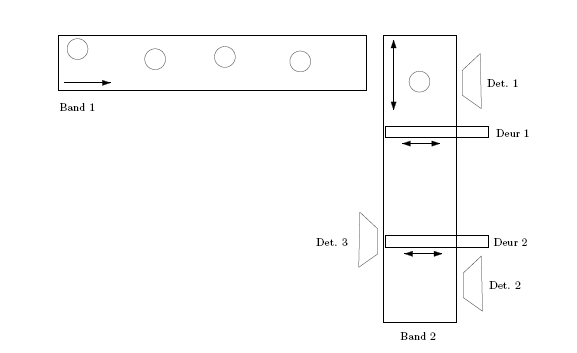
\includegraphics[width=0.8\linewidth]{schets}
\end{center}
\caption{Schema van de waferstepper}
\label{fig:schema}
\end{figure}

De belichtingsunit van de waferstepper is bereikbaar via een sluis
met twee deuren. Deze deuren mogen n\'{o}\'{o}it tegelijkertijd open
staan. Er zijn twee lopende banden. E\'{e}n waar te verwerken wafers
klaar liggen, deze kan maar \'{e}\'{e}n richting op, en \'{e}\'{e}n
waarop steeds een wafer door de deuren naar de belichtingsunit gaat
en weer terug. Wanneer een wafer bij de belichtingsunit komt, wordt
de band stilgezet, zodat de wafer belicht kan worden. Dit belichten
duurt precies twee seconden. Daarna gaat de wafer via de sluisdeuren
naar de verzamelbak.

Er bevinden zich twee licht detectoren in het systeem om de wafers
te lokaliseren. Deze detectoren bevinden zich aan de uiteinden van
de tweede band. Als er een wafer van de tweede band afvalt of af
wordt gehaald, dan wordt dit aangegeven door een extra led op het
processorbord te laten branden. Als er zo vijf wafers verloren gaan,
stopt het systeem en kan het alleen gerestart worden door een reset.

De wafers worden handmatig op de eerste band gelegd. Er is een
drukknop om aan te geven dat er wafers klaarliggen. Ook is er een
noodknop om het systeem te stoppen, en daarna weer te hervatten.

De waferstepper moet ten alle tijde aan de volgende voorwaarden
voldoen:
\begin{itemize}
  \item Wanneer de noodknop wordt ingedrukt stopt het systeem
  resoluut. Als de noodknop nu opnieuw wordt ingedrukt, hervat het
  systeem zijn oude taken, behalve als op zo'n moment een wafer belicht werd.
  Deze wafer is dan namelijk mislukt en zal niet opnieuw belicht worden.
  \item Beide sluisdeuren mogen nooit tegelijkertijd open staan,
  want dit zou de lens onherstelbaar beschadigen. Als een deur
  weigert te sluiten en dit gedetecteerd wordt door de sensor bij de
  deur, mag de andere deur dus niet opengaan.
  \item Wanneer er op de eerste band wafers klaar liggen en de ready
  button is ingedrukt, worden alle wafers zo snel mogelijk verwerkt en in de bak
  afgeleverd. Tenzij een wafer van de band valt. Het aantal van de band
  gevallen wafers komt overeen met het aantal brandende ledjes op het processorbord.
\end{itemize}
Verder geldt als algemeen design principe dat motoren,
luchtschakelaars en verlichting niet onnodig aangezet worden.

We maken eerst een systeemontwerp en bouwen de waferstepper. Hierna
maken we een programmaontwerp in UPPAAL. Met de Systeemanalyse
controleren we of het programmaontwerp goed werkt. Ten slotte
implementeren we het programmaontwerp in assembly, zodat we een
werkende waferstepper krijgen.


\begin{abstract}
\textbf{Tijdens dit OGO-project hebben we een waferstepper
nagemaakt. Een waferstepper is een machine die silicium wafers
belicht met UV-licht om er IC's van te maken. Dit belichten gebeurt
in een vacu\"{u}m, omdat UV-licht door de atmosfeer wordt
geabsorbeerd en omdat de lens kapot gaat wanneer deze aan de
buitenlucht wordt blootgesteld.}

\textbf{De waferstepper zelf hebben we gebouwd met behulp van
Fischertechnik. Hiermee zijn eenvoudig de echte loopbanden,
sluisdeuren, lamp en sensoren na te bootsen. We sturen de machine
aan met een processorbord met daarop een Siemens SAB-C504 processor.
Deze hebben we geprogrammeerd met assembleertaal. Voordat we de
processor geprogrammeerd hebben, hebben we een programmaontwerp
gemaakt en getest in UPPAAL.}

\end{abstract}
\clearpage


\chapter{Systeemontwerp}

\section{Inleiding van het systeemontwerp}
Het systeemontwerp beschrijft op een (betrekkelijk) abstract niveau
de opzet van ons ontwerp voor de Wafer stepper. Hierbij hebben wij
de aanwijzingen gevolgd uit het document ``Projectwijzer OGO1.3''.
Wij bespreken zowel de implementatie in het hardware model, als het
ontwerp in UPPAAL. Hierbij wordt nog niet uitgebreid ingegaan op de
software.


\section{Hardware}
\section{Opzet van het model}
We hebben ons systeem ingedeeld in de volgende onderdelen:
\begin{itemize}
    \item Lamp (UV en/of LED)
    \item Sensor
    \item Lopende Band (vooruit)
    \item Lopende Band (voor- en achteruit)
    \item Startknop
    \item Noodknop
    \item Deur
    \item FallOff**
    \item Luchtklep*
    \item Compressor*
    \item Pneumatische Cilinder*
    \item Bak (gelukt en afval)

\end{itemize}

De onderdelen gevolgd door ** kunnen niet in het hardware model worden opgenomen, dit zijn geen fysieke componenten. \\
De onderdelen gevolgd door * zijn niet opgenomen in het UPPAAL model. Onder andere omdat ze altijd aan moeten zijn, of door een ander onderdeel, dat w\'el gemodelleerd is, bestuurd worden. \\ \\

Hieronder bespreken wij alle onderdelen aan de hand van foto's van ons model. Hierbij hebben wij gebruik gemaakt van foto's waarbij, na omcirkeling, een onderdeel nog herkenbaar is. \\ \\

Wegens de conversie door \LaTeX bij het invoeren van plaatjes met transparency, zijn er zwarte vlakken om onze foto's ontstaan. Onze excuses voor eventuele ongemak.


\section{Foto's van het model}\label{sec:foto_s_van_het_model} % (fold)

\subsection{Lamp}\label{sub:Lamp} % (fold)


  
\includegraphics[width=13cm, height=11cm]{lamp} \\
  \includegraphics[width=13cm, height=8cm]{UVlamp} \\

Op deze foto's zijn de eerste LED respectievelijk de UV-lamp te zien.
De tweede LED kan niet worden gefotografeerd wegens obstructies. \\
Tegenover de twee LED's staat bij ieder \'e\'en sensor, deze worden hierna behandeld.


% subsection lamp (end)

\subsection{Sensor}\label{sub:sensor} % (fold)
  
\includegraphics[width=13cm, height=14cm]{lamp} \\
  \includegraphics[width=13cm, height=9cm]{UVlamp} \\
  Op de foto's zijn sensor 1 respectievelijk sensor 2 weergegeven, om te illustreren hoe deze zijn ge\"implementeerd in het hardware model.

  In totaal maken wij gebruik van vier sensoren, namelijk:
  \begin{itemize}
    \item R1, deze sensor ``ziet'' de wafer voor de eerste deur
    \item R2, deze sensor ``ziet'' de wafer achter de tweede deur
    \item D1, deze sensor bevestigt het sluiten van deur 1
    \item D2, deze sensor bevestigt het sluiten van deur 1
  \end{itemize}
% subsection sensor (end)


\subsection{Lopende band (vooruit)}\label{sub:lopende_band_vooruit_} % (fold)
  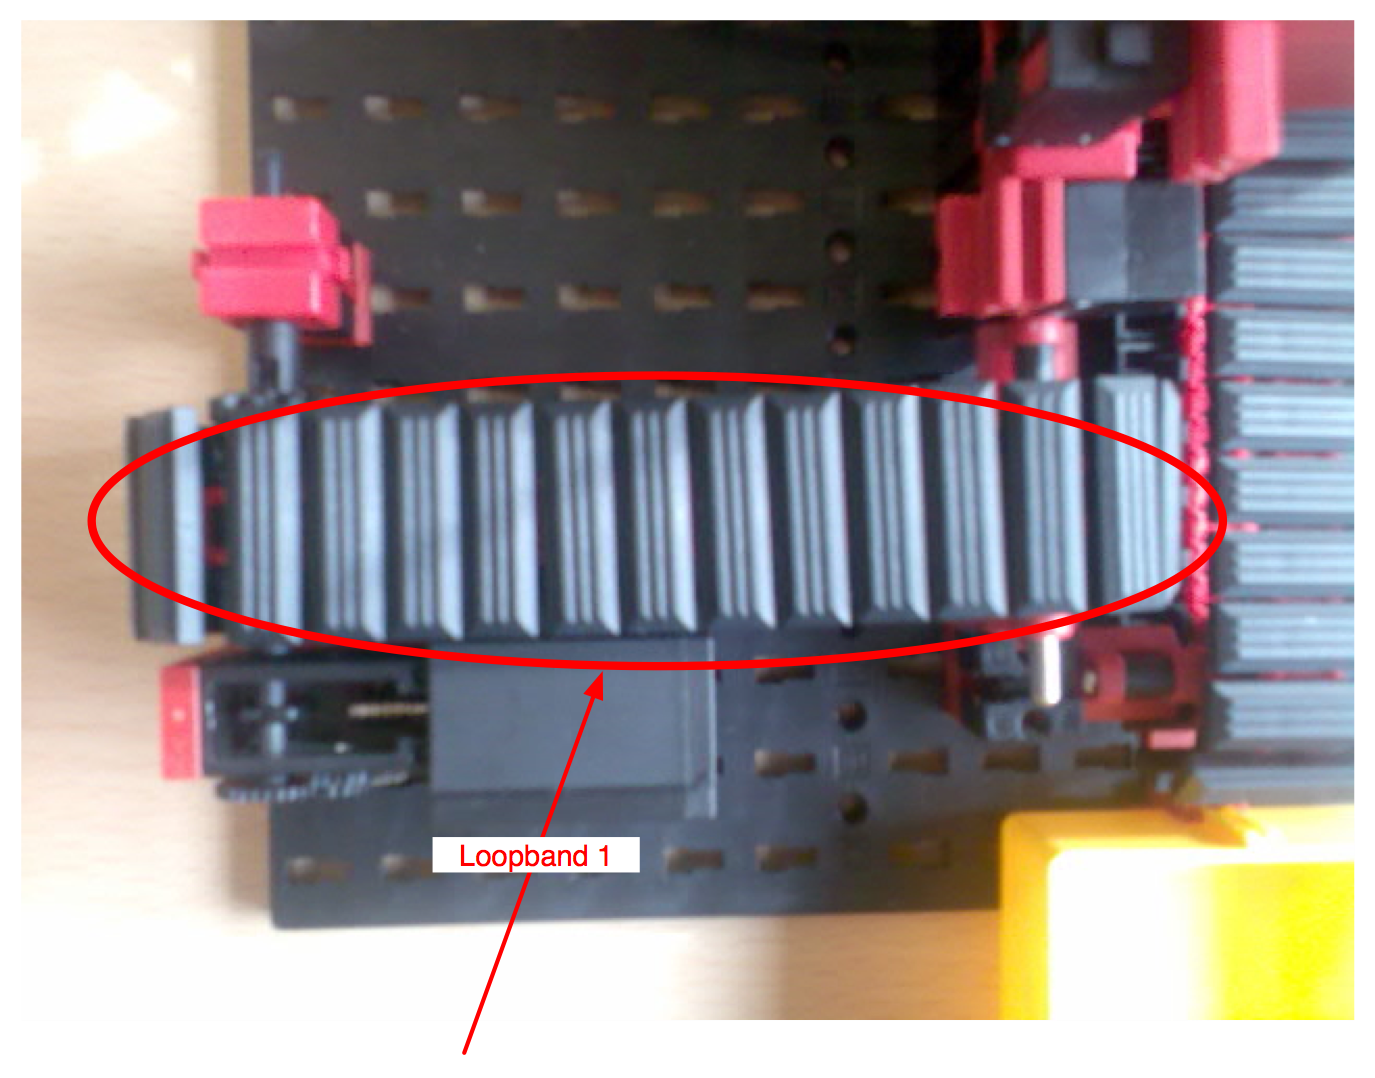
\includegraphics[width=13cm, height=14cm]{LB1} \\

  Dit is de lopende band die de wafers aanlevert. Deze kan alleen vooruit lopen. \\
  Het grote blok ten hoogte van het midden van de band is de motor die deze loopband aandrijft.
% subsection lopende_band_vooruit_ (end)

\subsection{Lopende band (vooruit)}\label{sub:lopende_band_vooruit_} % (fold)
  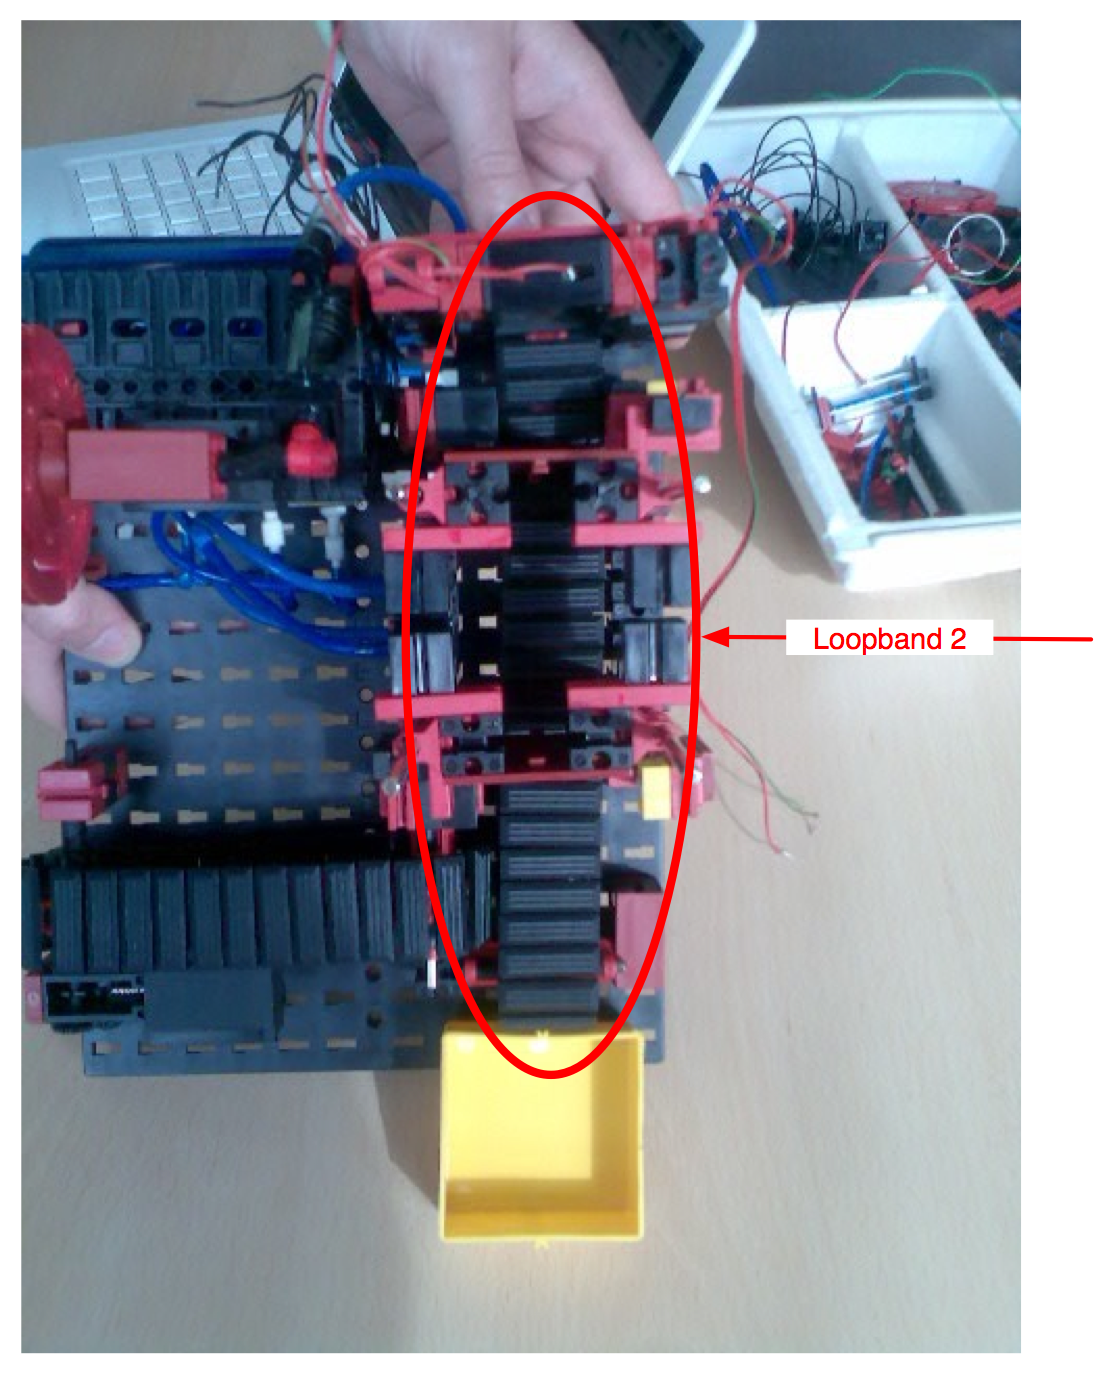
\includegraphics[width=13cm, height=14cm]{LB2} \\

  Dit is de lopende band die de wafers door de twee poorten brengt. Deze band kan voor- en achteruit. \\
   De motor die deze loopband aandrijft is meegenomen in de structuur van het model. Deze maakt deel uit van de pilaar waar de UV-lamp op hangt. Hierdoor hebben wij geen duidelijke foto kunnen maken van de aandrijfmotor.
% subsection lopende_band_vooruit_ (end)

\subsection{Knoppen}\label{sub:knop} % (fold)
  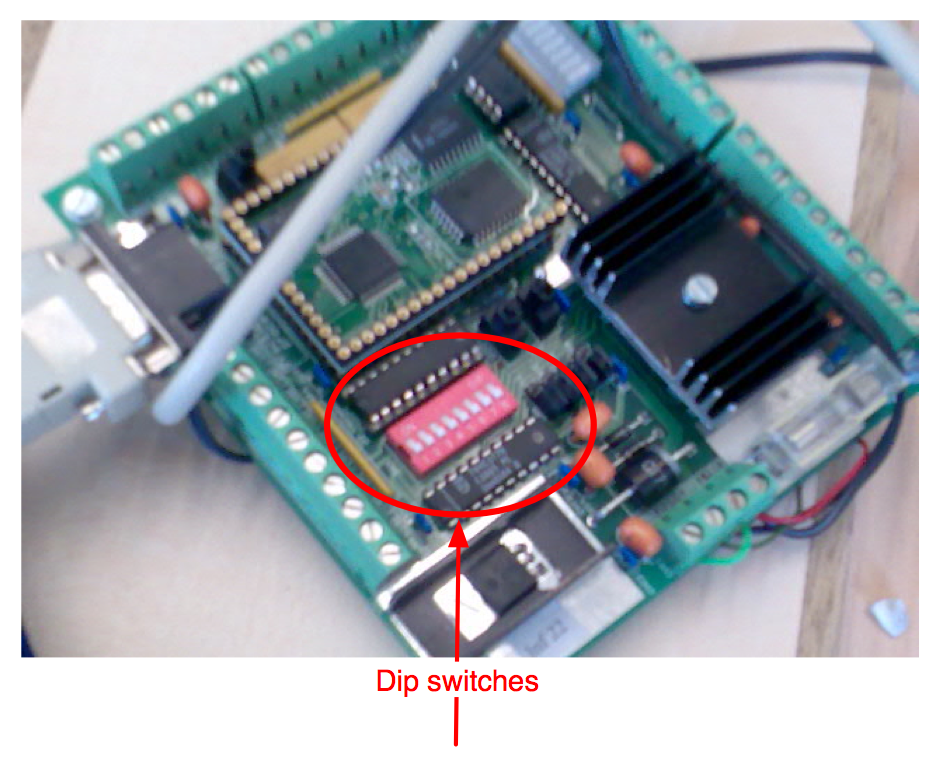
\includegraphics[width=13cm, height=14cm]{dip} \\
  Wij maken gebruik van een DIP-switch, op het geleverde processor bord, als
  startknop. Als noodknop hebben we een aparte knop maar hier is
  geen foto van.
% subsection knop (end)

\subsection{Deur}\label{sub:deur} % (fold)
  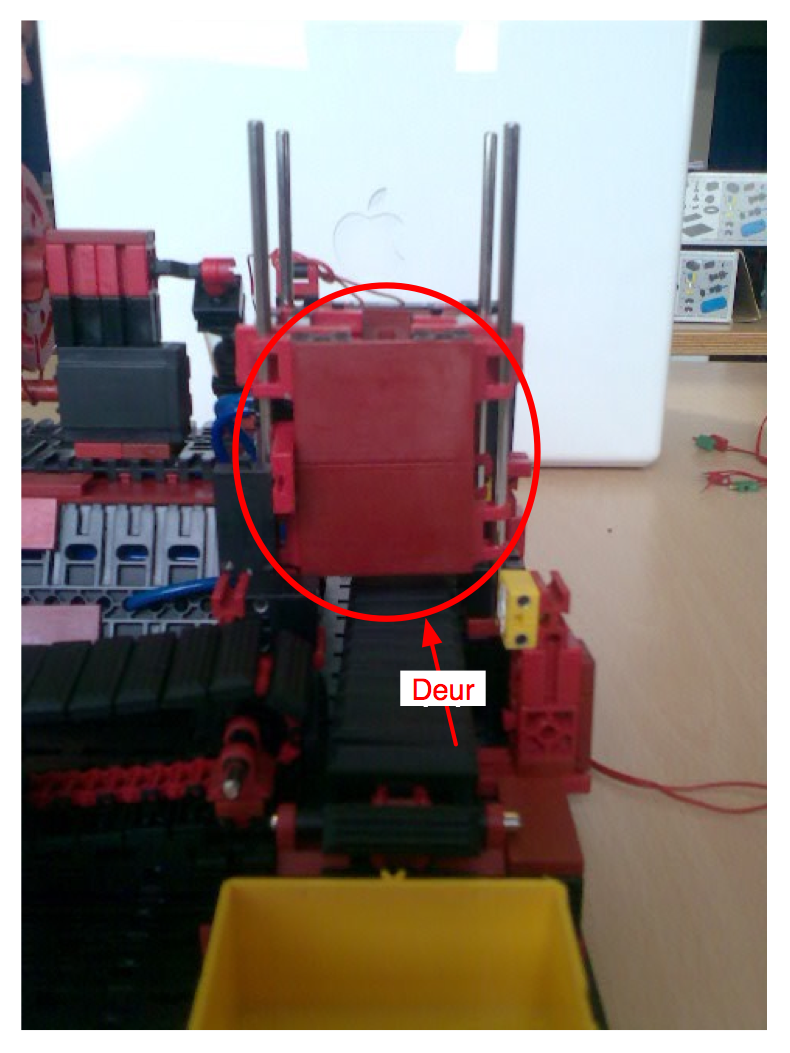
\includegraphics[width=13cm, height=14cm]{deuren_voor} \\
  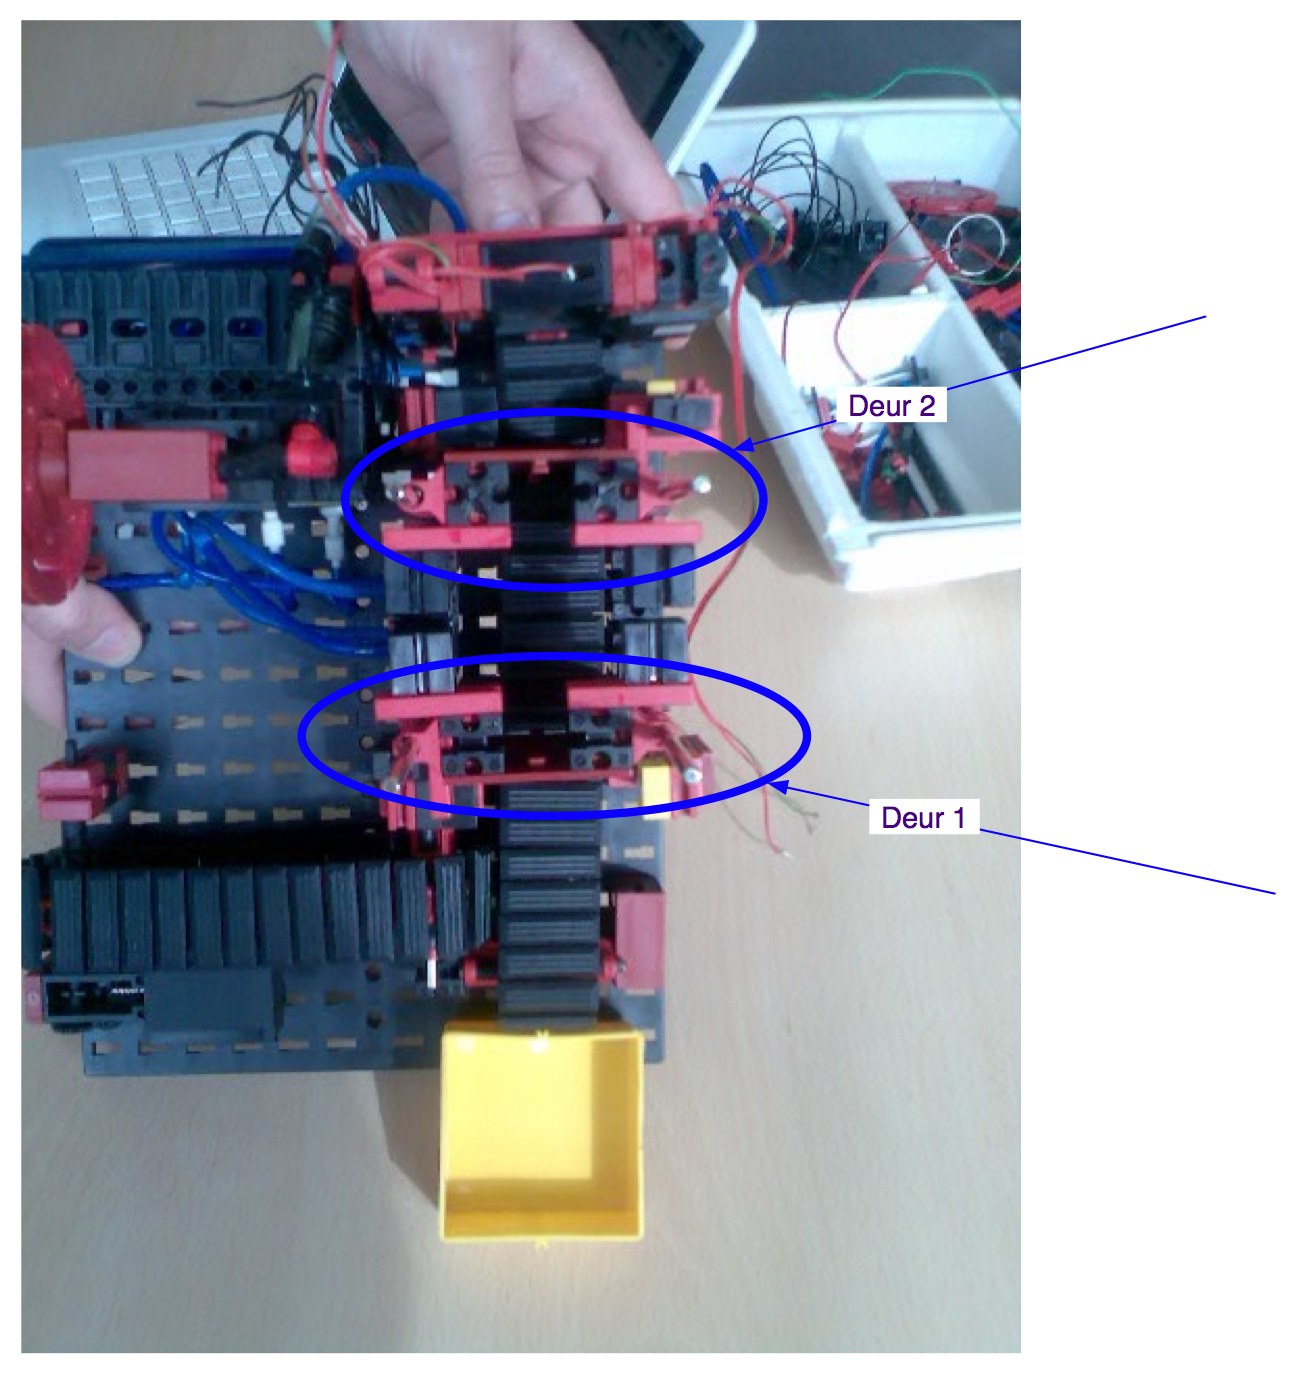
\includegraphics[width=13cm, height=14cm]{deuren} \\

Een voor en boven aanzicht van de twee deuren die de UV-lamp van de
buitenwereld scheiden, zodat deze niet beschadigd kan worden. Wegen
obstructie is er geen vooraanzicht foto van de tweede deur.

% subsection deur (end)


\subsection{Luchtkleppen}\label{sub:luchtkleppen} % (fold)
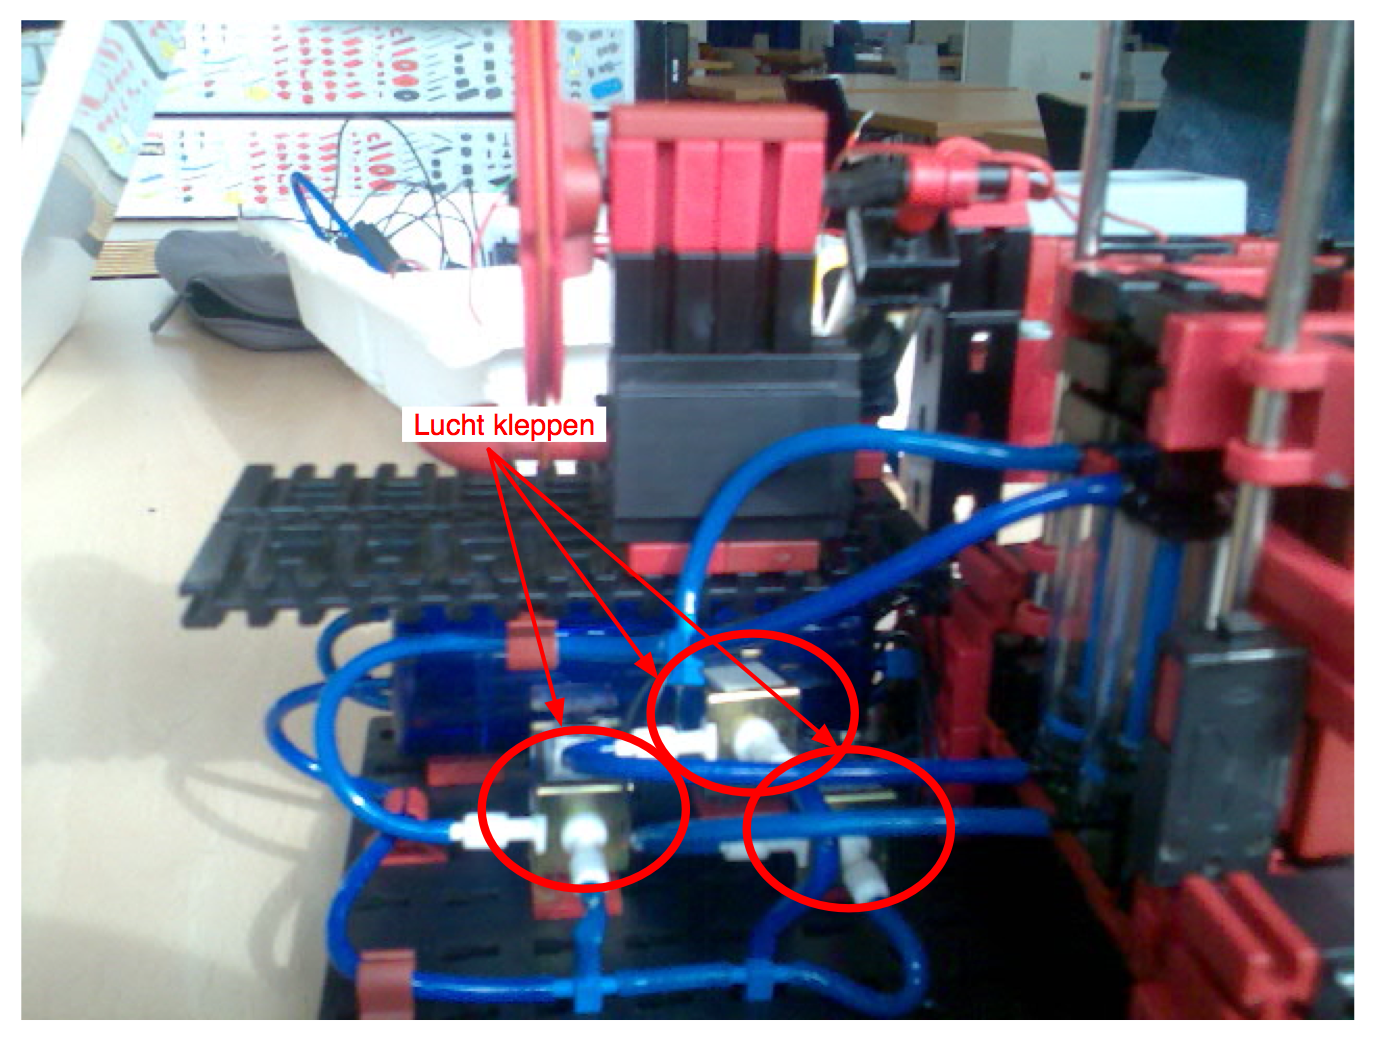
\includegraphics[width=13cm, height=14cm]{valve} \\
Drie van de vier luchtkleppen die gebruikt worden om lucht wel of niet door te laten. De vierde luchtklep is na het maken van deze foto geplaatst, bij de andere drie. Er is hier geen afbeelding van.

% subsection luchtkleppen (end)

\subsection{Compressor}\label{sub:compressor} % (fold)

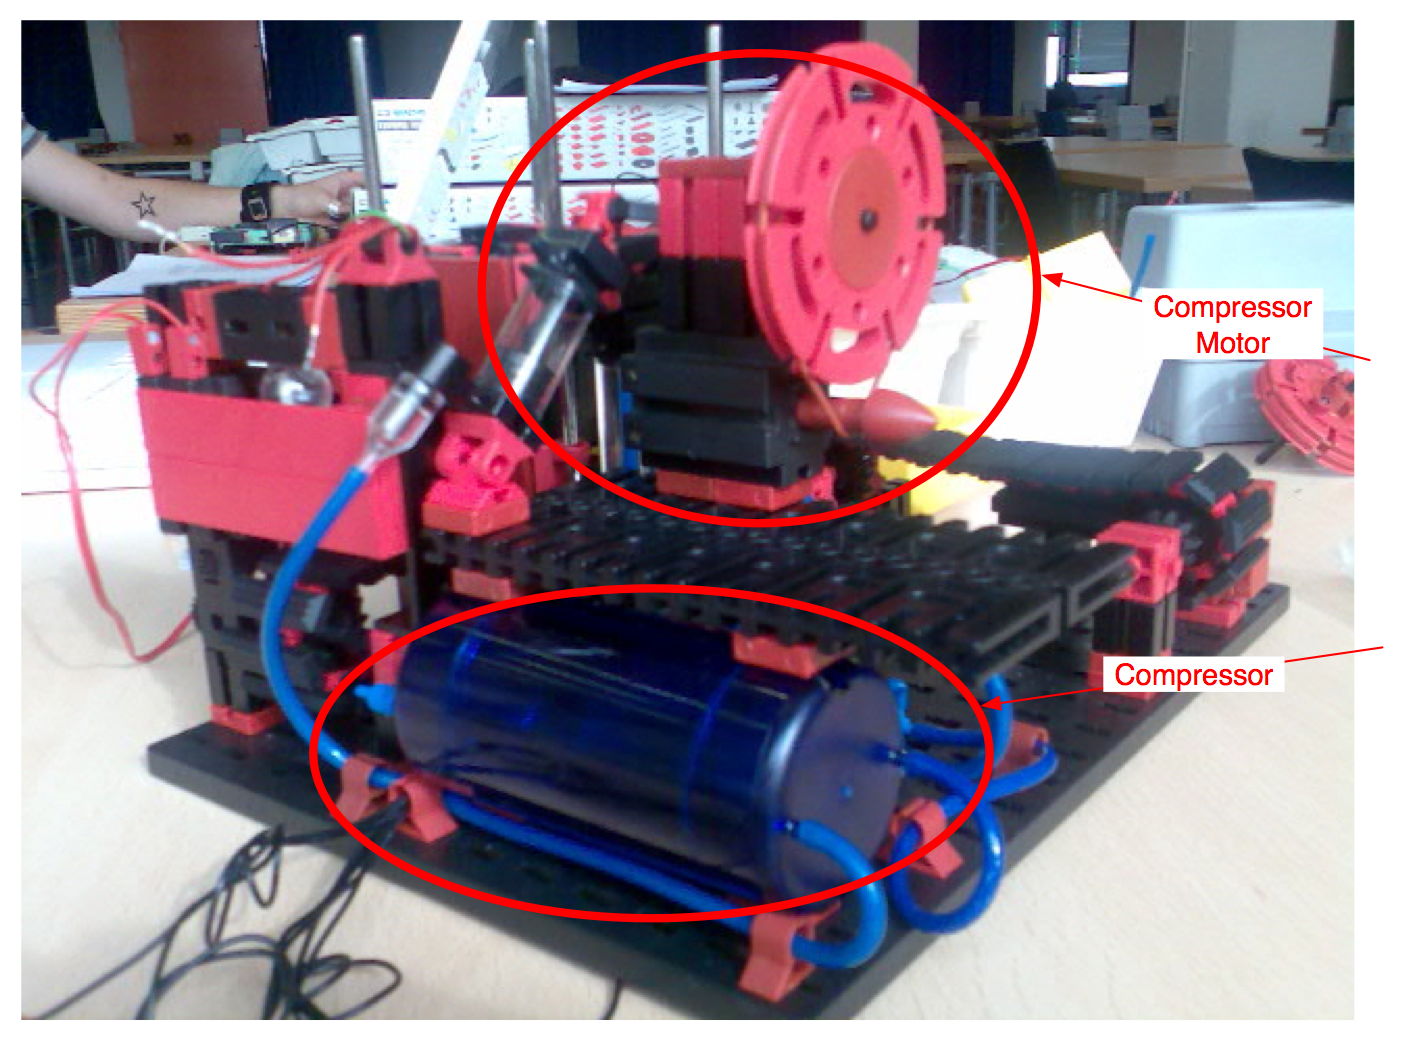
\includegraphics[width=13cm, height=14cm]{compressor} \\
De compressor en de motor die de compressor vult. Deze begint met
draaien zodra het model ingeplugd wordt op het net-stroom. De
compressor en diens motor draaien geheel onafhankelijk van alle
andere onderdelen en kunnen niet worden be\"invloed door de
processor.

% subsection compressor (end)



\subsection{Pnematische Cilinder}\label{sub:pnematische_cilinder} % (fold)

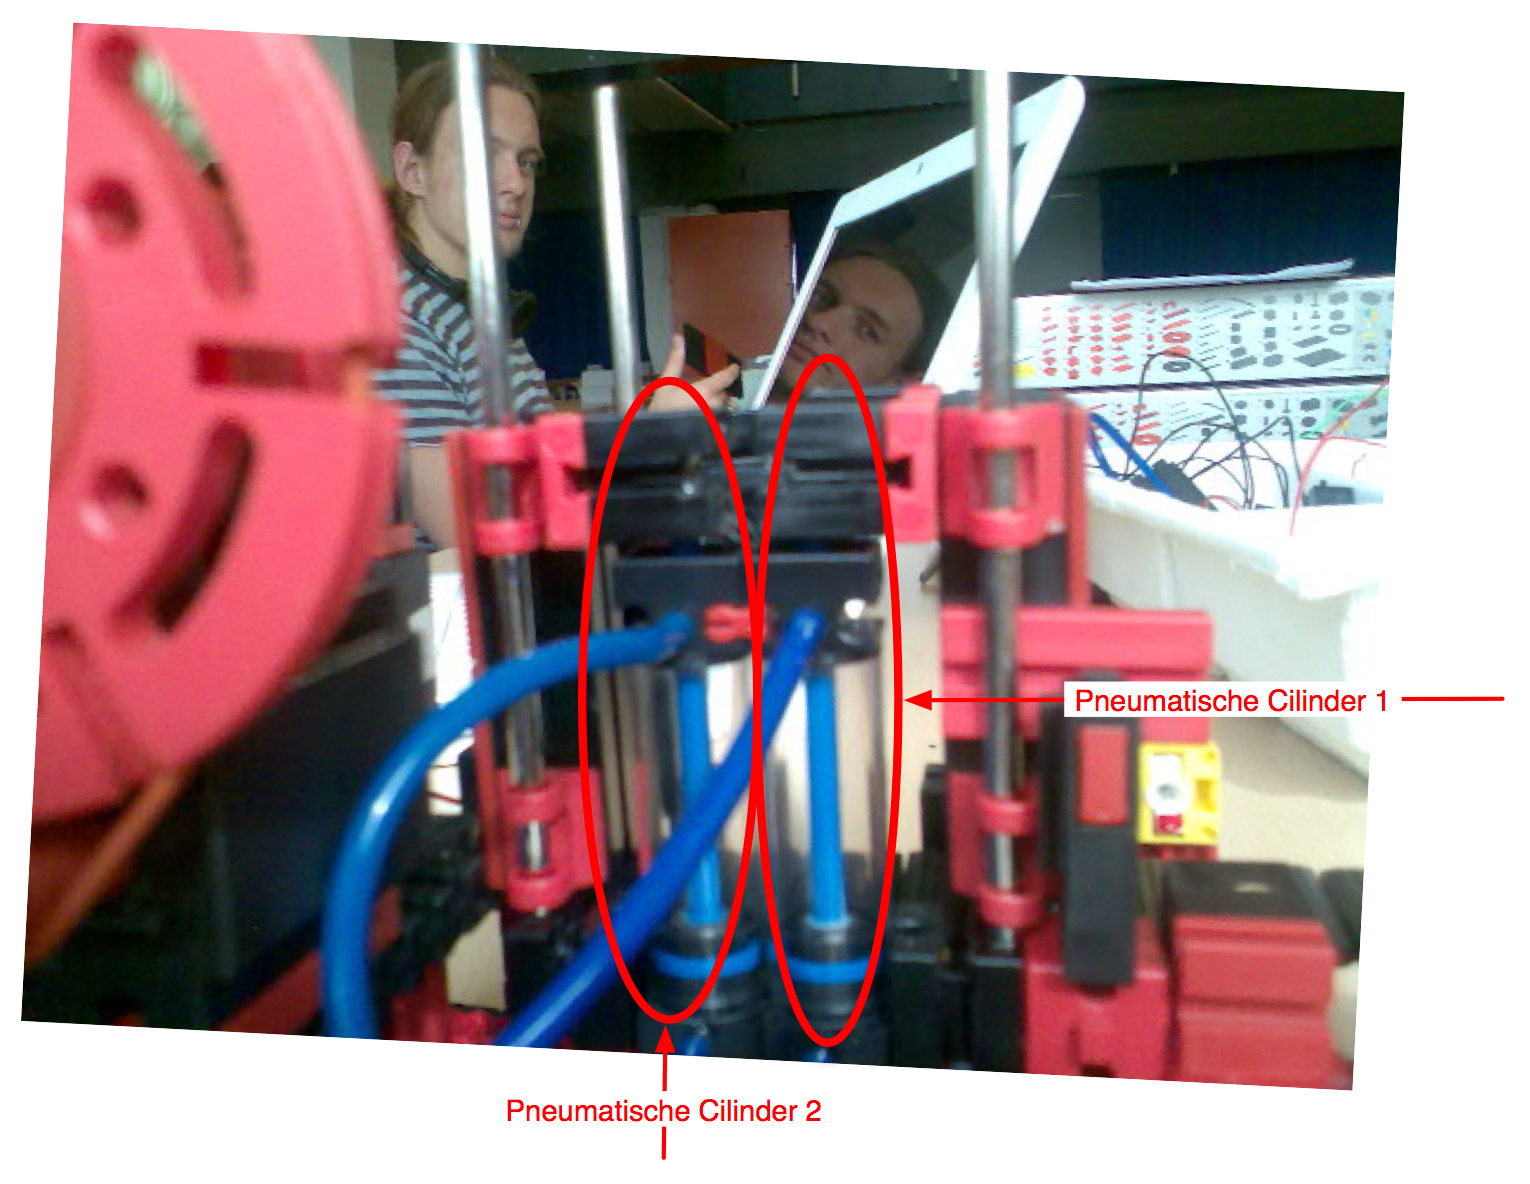
\includegraphics[width=15cm, height=11cm]{PC} \\
De pneumatische cilinder duwt de deur omhoog en trekt hem ook weer omlaag. Wij maken gebruik van twee cilinders, ieder voor \'e\'en deur. De cilinders worden door de luchtkleppen aangestuurd en zijn daarom niet in het UPPAAL model opgenomen.

% subsection pnematische_cilinder (end)

\subsection{Bak}\label{sub:bak} % (fold)

\includegraphics[width=13cm, height=14cm]{lamp} \\
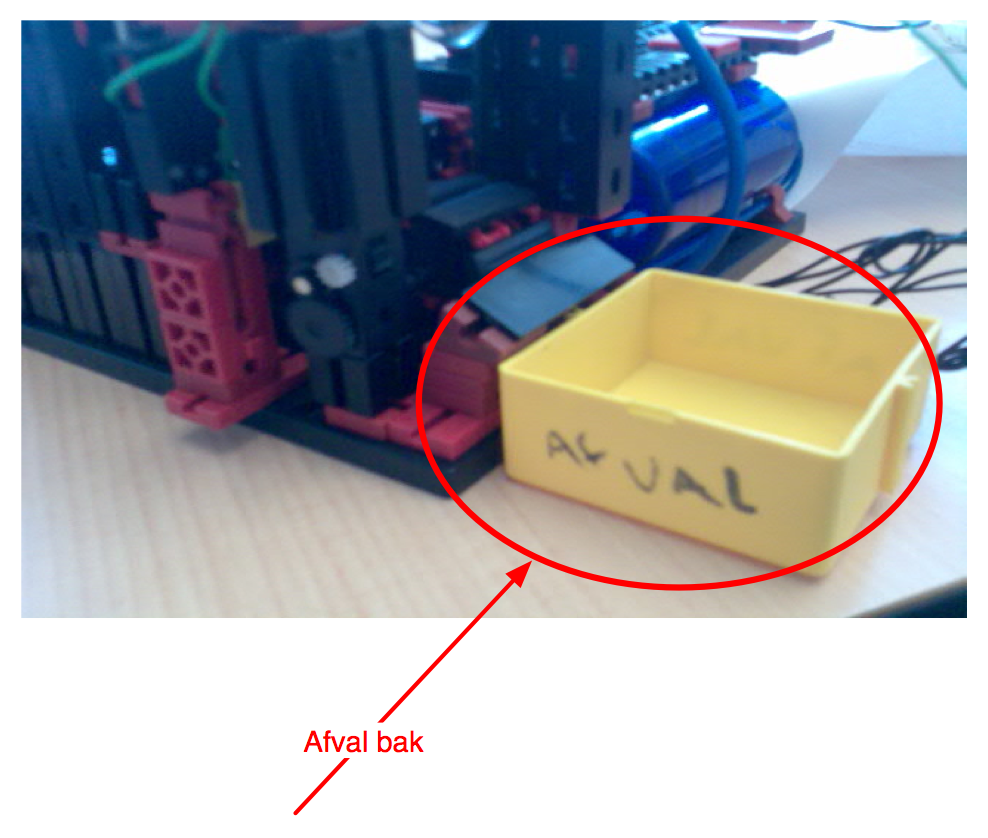
\includegraphics[width=13cm, height=11cm]{afval} \\

De twee bakken voor de gelukte wafers en de afval bak. De afval bak
staat het dichtst bij de UV-lamp. De bak voor de gelukte wafers
staat ver weg van de UV-lamp, voorbij de twee deuren en ter hoogte
van waar de volgende wafer wordt aangeleverd.

% subsection bak (end)

% section foto_s_van_het_model (end)
\section{Ontwerpbeslissingen}
Wij maken gebruik van twee fysieke deuren, die helemaal dicht zijn
en voorkomen dat er een wafer voorbij onze deur komt.
Onze deur wordt omhoog geduwd door 1 cilinder per deur. Dit leek ons het meest logische, een deur die van boven af wordt bestuurd houdt in dat je de luchtkleppen zou moeten inverteren (dicht is dan de valve aan zetten). Een tweede cilinder om de deur omhoog te duwen werkt niet, onze compressor kan daar niet genoeg druk voor opbouwen. Daarom maken wij gebruik van stalen staafjes waar de deuren makkelijk over glijden. \\ \\

Wij hebben besloten om een wafer die mislukt is (omdat er tijdens het bestralen op de noodknop is gedrukt) in een andere bak te deponeren, de afval bak. Hoewel het makkelijker is om de wafer te behandelen als een normale wafer, is het logischer om deze wafers apart te houden, ze zijn immers onbruikbaar. \\ \\

Wij hebben ervoor gekozen om beiden deuren apart aan te sturen. Het is namelijk mogelijk om \'e\'en luchtklep aan te sluiten aan beide deuren, zodat deze beiden tegelijkertijd sluiten. Omwille van mogelijk onderhoud dat gepleegd zou kunnen worden bij een echte wafer stepper, hebben wij ervoor gekozen omdat beiden deur onafhankelijk van elkaar aan te sturen. \\ \\

Wij maken gebruik van twee druksensoren om te kijken of deur dicht is. Hoewel aangekondigd was dat er niet genoeg druksensoren waren om beiden deuren te controleren, hadden wij in onze dozen twee druksensoren. De zijn beiden gekoppeld aan de onderkant van de deur. Beiden deuren hebben een uitsteekseltje om de druksensor te activeren indien de deur dicht is. \\ \\




\chapter{UPPAAL model}\label{chap:uppaal_model} % (fold)


% section uppaal_model (end)

Dit zijn al onze UPPAAL componenten. \textit{Opmerking:} deze
versies van ProgramInit en ProgramRun zijn verouderd. Hierdoor
kloppen een paar dingen niet meer. Zo waren bPress[1] en bRelease[1]
eerst kanalen die aangaven dat de noodknop ingedrukt respectievelijk
losgelaten werd, maar zijn er nu een nieuwe noodknop-template en
daardoor (handigere) emStart en emStop kanalen. Zie voor een goede
versie van het hoofdprogramma het programmaontwerp.

\begin{itemize}
    \item ``ProgramInit'' wordt aan het begin van het programma uitgevoerd. Dit zorgt ervoor dat alle actoren in een wenselijke toestand zijn. Als ProgramInit klaar is, wordt ProgramRun aangeroepen. \textit{Opmerking:} we mogen
    er van uit gaan dat alles in het begin in de wenselijke toestand is, dit hebben we in het programmaontwerp dan ook gedaan, waardoor daar geen ProgramInit of equivalent daarvan te vinden is. \\
    \textbf{Program Init} \\
    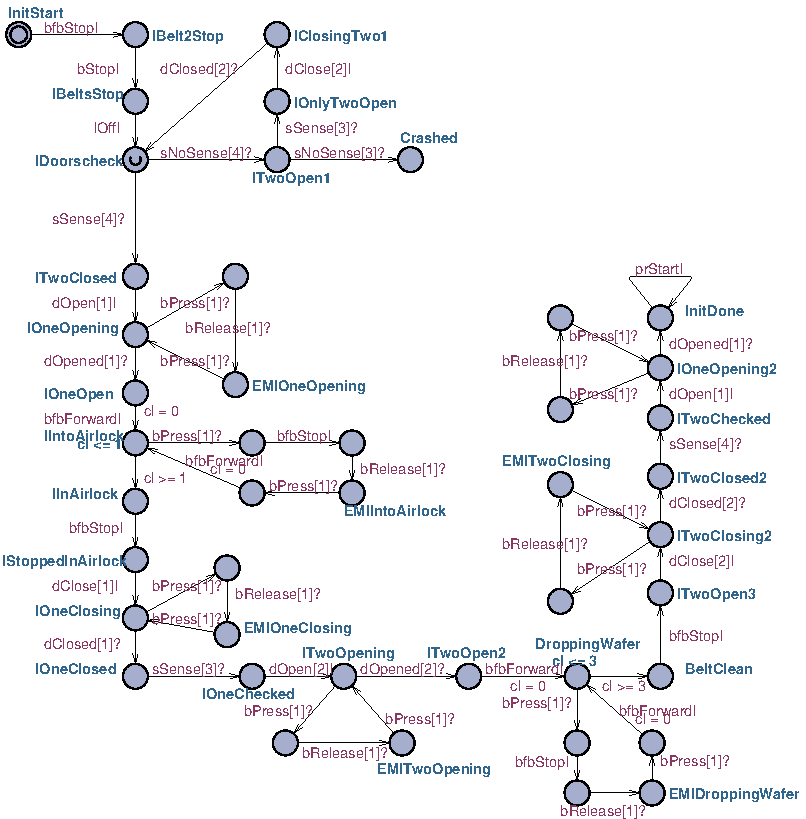
\includegraphics[scale=.7]{ProgramInit} \\
    \textbf{Program Run} \\
    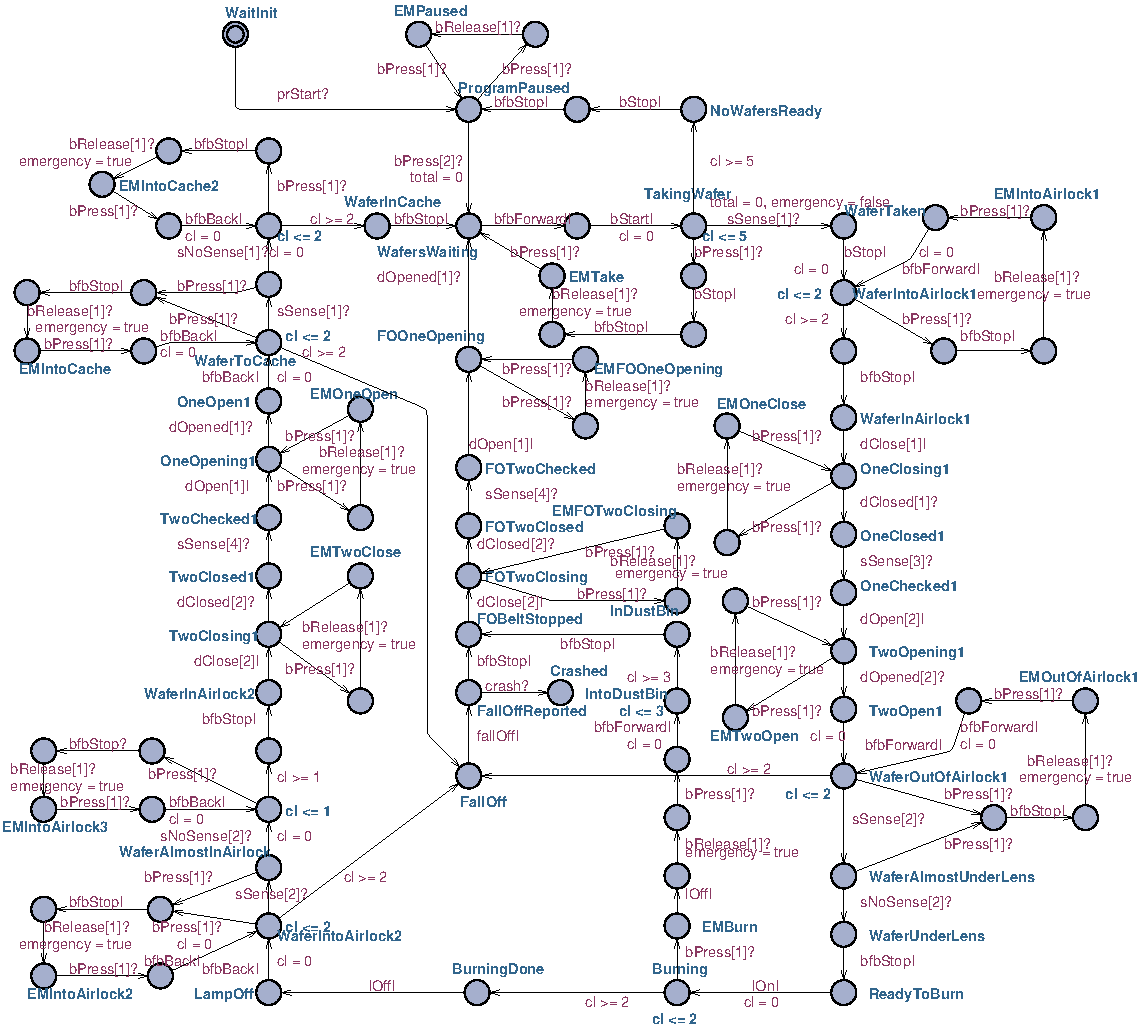
\includegraphics[scale=.7]{ProgramRun} \\
    \item ``StartButton'' staat voor de startknop. Deze kan alleen ingedrukt worden, er wordt dan een signaal verstuurd waardoor het systeem start.  \\
    \textbf{StartButton} \\
    
\includegraphics{UPstartbutton} \\
    \item ``EMButton'' staat voor de noodknop. Hier zijn drie toestanden mogelijk. E\'{e}n toestand stelt een emergency voor, \'{e}\'{e}n
    toestand wordt bereikt als het systeem uit een emergency komt en de laatste toestand zorgt ervoor dat het systeem niet gelijk weer in emergency
    kan gaan als een emergency afgelopen is. \\
    \textbf{EMButton} \\
    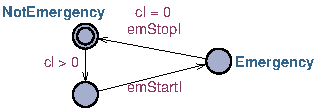
\includegraphics{UPEMbutton} \\
    \item ``Lamp'' staat voor een LED of de UV-lamp. Deze kan aan of uit staan. \\
    \textbf{Lamp} \\
    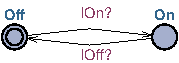
\includegraphics{UPlamp} \\
    \item ``Conveyor'' is de lopende band die maar 1 kant op kan lopen. Deze kan dus 'aan' (running) of 'uit' (stopped) zijn.\\
    \textbf{Conveyor} \\
    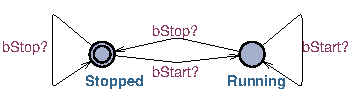
\includegraphics{UPconveyor} \\

    \item ``ConveyorBF'' kan heen en terug lopen. Er zijn dus toestanden voor back, forward en stopped nodig.\\
    \textbf{ConveyorBF} \\
    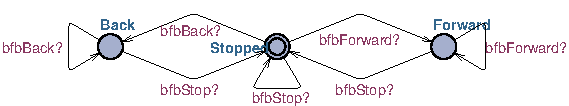
\includegraphics{UPconveyorBF} \\
    \item ``Door'' is het model van een deur. Een deur kan open of dicht zijn. Als een geopende deur een open-signaal krijgt (of een gesloten deur een sluit-signaal), dan wordt dit verwerkt door meteen aan te geven dat de deur klaar is met openen (of sluiten).\\

    \textbf{Door} \\
    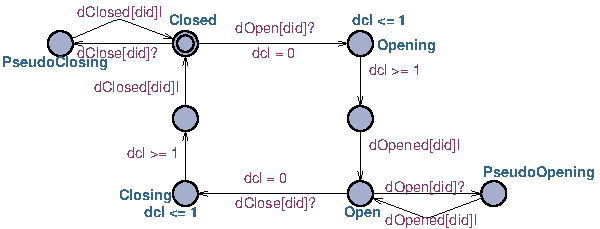
\includegraphics{UPdoor} \\
    \item ``Sensor'' is een licht- of druksensor. Een sensor kan Sense of NoSense zijn - hij neemt iets waar of hij neemt niets waar.\\
    \textbf{Sensor} \\
    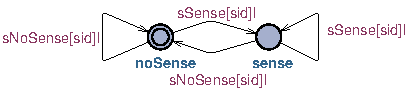
\includegraphics{UPsensor} \\
    \item ``FallOff'' - dit is een speciaal geval. Het is niet echt een hardware-component (ondanks dat er wel LEDs aan en uit gaan ten gevolge van de toestand van dit onderdeel). FallOff houdt bij hoeveel wafers van de band gevallen zijn. Zodra er vijf wafers verloren zijn gegaan 'crasht' ons systeem (dit is een noodtoestand). We houden dit op deze manier bij omdat de hoeveelheid verloren wafers van groot belang is voor de werking van het systeem.\\
    \textbf{falloff} \\
    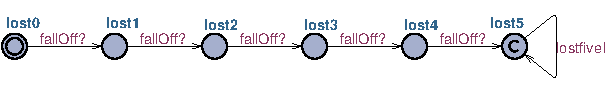
\includegraphics{UPfalloff} \\
\end{itemize}

Veel van de componenten hebben een onbekende beginstand, een gegeven dat gemodelleerd is door vanuit Init een stap te maken naar een willekeurige toestand.\\
Daarnaast wordt van veel componenten verwacht dat ze een signaal kunnen versturen,  (``deze deur staat open!'') - dit wordt gedaan door in elke  'stabiele' toestand (de deur staat open) een loopje naar dezelfde toestand te maken. Deze loop verstuurt een signaal over het gewenste kanaal.



\section{Ontwerp Beslissingen}\label{sec:ontwerp_beslissingen} % (fold)

We hebben expliciet gekozen om geen wafer-element toe te voegen. Dit
zou namelijk betekenen dat de wafers zelf te besturen zijn, iets dat
niet zo is. Er is helemaal niets bekend over de wafer, alleen over
het feit dat sensoren iets registreren of niet. Uit deze informatie
kan dan weer worden afgeleid waar een wafer is.\\ \\

``FallOff'' is expliciet gedeclareerd omdat er bepaalde lampjes zijn
die overeenkomen met een aantal wafers die weg zijn. Elke toestand van
``FallOff'' bestuurd nu impliciet die lampjes. Daarnaast is het zo dat
zodra de vijfde wafer van de band af valt er een noodstop gemaakt
moet worden. \\ \\


% chapter ontwerp_beslissingen (end)










%Al deze onderdelen spreken voor zich, behalve de Teller. Dit element
%houdt bij hoeveel wafers er van de band afgevallen zijn. De
%onderdelen hebben hun eigen template en mogelijkheden om te
%communiceren met de buitenwereld. Hierdoor kunnen orders gegeven
%worden aan actoren en de staat van sensoren gelezen worden.
%
%
%\section{Ontwerpbeslissingen}
%

%



\chapter{Specificatie elektrische interface}
\section{Priklijst}

    \vspace{-6em}

    \begin{center}
    \includegraphics[scale=.7]{priklijst1}
    \vspace{-6em}
    \includegraphics[scale=.7]{priklijst2}
    \end{center}


\section{Bedradingsschema}


    %\begin{figure}
    \begin{center}
    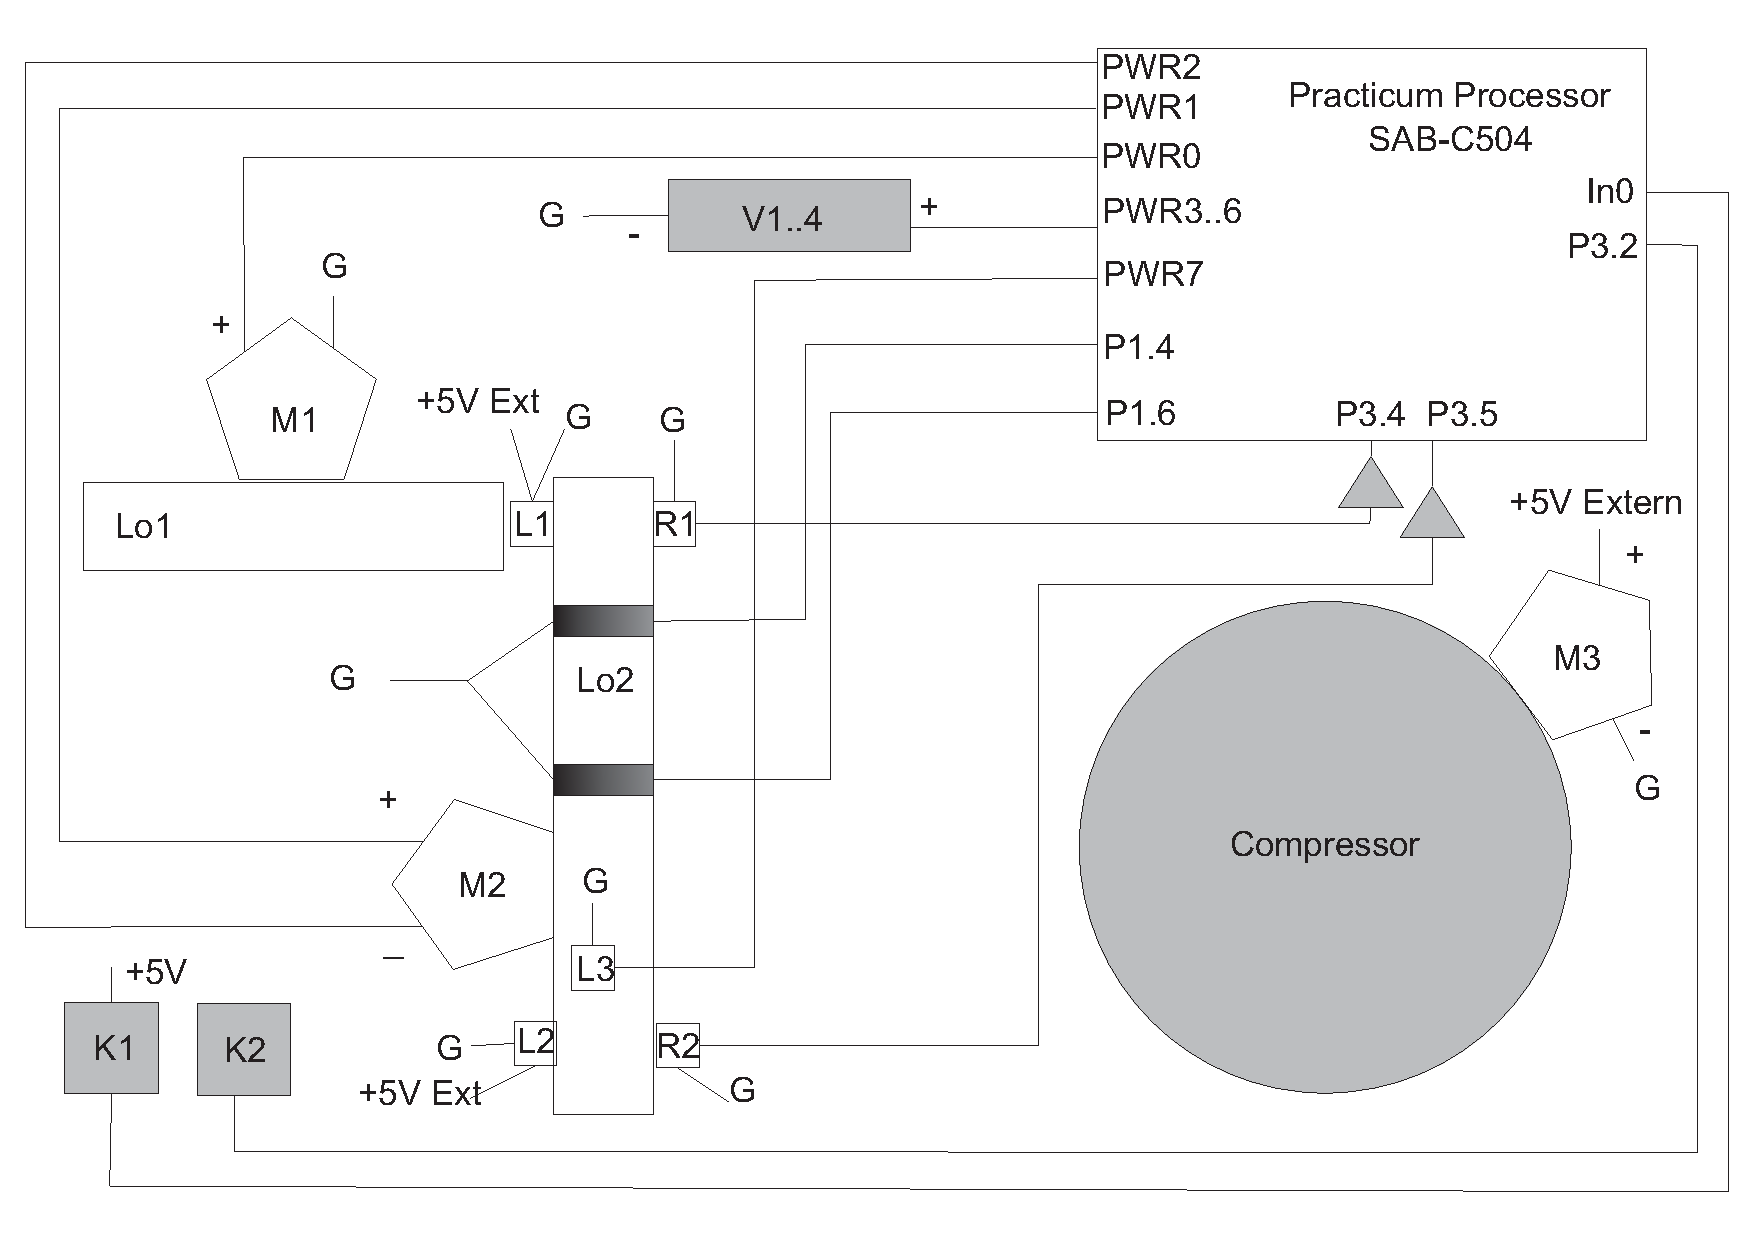
\includegraphics[scale=.5]{bedrading}
    \end{center}
    %\end{figure}

\section{Beluchtingsschema}


    %\begin{figure}
    \begin{center}
    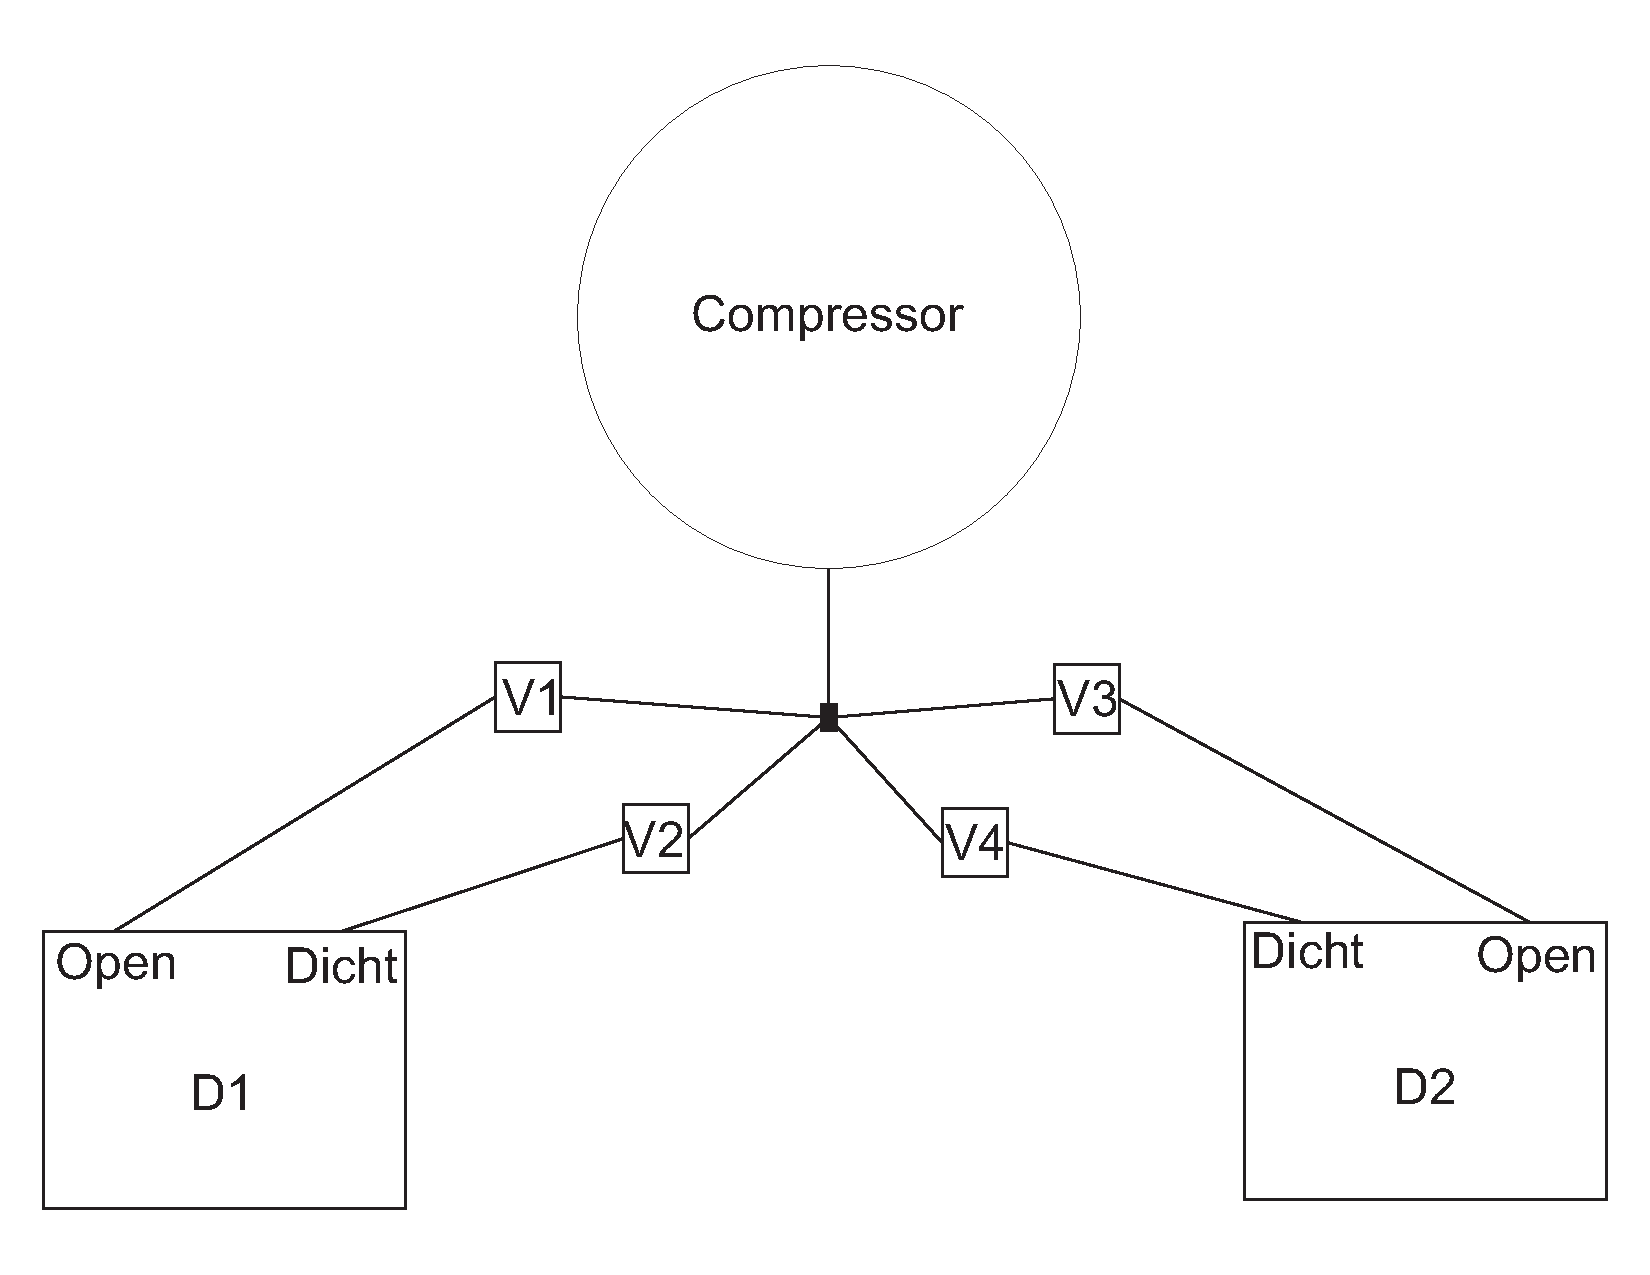
\includegraphics[scale=.5]{beluchting}
    \end{center}
    %\end{figure}

    We gebruiken \'{e}\'{e}n compressor waarop vier luchtkleppen zijn
    aangesloten. E\'{e}n luchtklep dient om deur 1 te openen,
    \'{e}\'{e}n om deur \'{e}\'{e}n te sluiten, er is er \'{e}\'{e}n om deur twee
    te openen, de laatste sluit deur twee. We hebben overwogen om
    \'{e}\'{e}n luchtklep te gebruiken om beide deuren te sluiten,
    omdat toch nooit beide deuren gelijk open mogen zijn. We hadden
    toen echter ons beluchtingsschema al ingeleverd en hebben het
    dus maar bij het originele ontwerp gelaten.


\chapter{Programmaontwerp}
\documentclass[]{report}
%% Gebruikte pakketten
\usepackage[dutch]{babel}
\usepackage{geometry}
\usepackage{graphicx}
\usepackage{amssymb}
\usepackage{epstopdf}
\usepackage{textcomp}
\usepackage[]{hyperref}
\usepackage{fancyhdr}

\title{Programmaontwerp verslag UPPAAL}
\author{Groep 7 OGO 1.3 2006-2007}
\date{05-22-2007}


\begin{document}
  %%%%%%%%%%%%%%%%%%%%%%%%%%%%%%%%%%%%%%%%%%%%%%%%%%%%%%%%%%%%%%%%%
% Contents: The title page
% $Id: title.tex,v 1.2 2003/03/19 20:57:47 oetiker Exp $
%%%%%%%%%%%%%%%%%%%%%%%%%%%%%%%%%%%%%%%%%%%%%%%%%%%%%%%%%%%%%%%%%
\ifx\pdfoutput\undefined % We're not running pdftex
\else
\pdfbookmark{Titelblad}{title} \fi
\newlength{\centeroffset}
\setlength{\centeroffset}{-0.5\oddsidemargin}
\addtolength{\centeroffset}{0.5\evensidemargin}
%\addtolength{\textwidth}{-\centeroffset}
\thispagestyle{empty}
\vspace*{\stretch{1}}
\noindent\hspace*{\centeroffset}\makebox[0pt][l]{\begin{minipage}{\textwidth}
\flushright
{\Huge\bfseries Wafer stepper\\
                  <verslag> \\}
\noindent\rule[-1ex]{\textwidth}{5pt}\\[2.5ex]
\hfill\emph{\Large OGO 1.3: Groep 7}
\end{minipage}}

\vspace{\stretch{1}}
\noindent\hspace*{\centeroffset}\makebox[0pt][l]{\begin{minipage}{\textwidth}
\flushright
{\bfseries
door: \\ \newline
\begin{tabular}{ r | c}
  \multicolumn{2}{c}{ } \\
  Etienne van Delden & 0618959  \\
  Gijs Direks        & 0611093  \\
  Sanne Ernst        & 0588898  \\
  Bas Goorden        & 0598669  \\
  Stef Sijben        & 0607426  \\ 
  Coen van der Wel   & 0608467  \\

\end{tabular}\\ [3ex]}
<datum>
\end{minipage}}

%\addtolength{\textwidth}{\centeroffset}
\vspace{\stretch{2}}



\endinput

  \tableofcontents

    \chapter{Inleiding}
        Het programmaontwerp is een netwerk van UPPAAL-automaten die
        beschrijven hoe het gedrag van het programma dat de
        waferstepper aanstuurt hoort te zijn. In dit document zullen
        we beschrijven hoe we dit netwerk van automaten gemodelleerd
        hebben en waarom we dat op deze manier gedaan hebben.


        We gaan er in dit verslag vanuit dat alle aangesloten apparaten
        een nette begintoestand hebben, dat wil zeggen: de deuren zijn
        gesloten, lopende banden staan stil, de lamp voor het belichten
        is uit en sensors rapporteren niets.


    \chapter{Het UPPAAL ontwerp voor de subroutines}
        Het UPPAAL ontwerp is verdeeld in verschillende templates
        die allemaal verantwoordelijk zijn voor een bepaalde actie
        en daarnaast een template die alle anderen aanstuurt. Al
        deze templates zullen in dit hoofdstuk beschreven worden,
        behalve die van het hoofdprogramma, die in het volgende
        hoofdstuk aan bod komt.\\

        De templates in dit hoofdstuk maken gebruik van de templates
        uit het ontwerpverslag, die de daadwerkelijke hardware
        modelleeren.

    \section{Bediening lopende banden}
        Er zijn in ons programmaontwerp een zevental automaten die
        op een bepaalde manier een lopende band aansturen, die weer
        verder verdeeld kunnen worden in drie groepen:
        \begin{itemize}
            \item Gedurende een bepaalde tijd loopband 2 voor- of
            achteruit bewegen
            \item Loopband twee voor- of achteruit bewegen totdat
            een sensor iets ziet of totdat er een time-out optreedt
            \item Een wafer van de eerste loopband proberen te
            pakken en op loopband twee te leggen.
        \end{itemize}

    \subsection{Een bepaalde tijd bewegen: MoveBackwardT en
    MoveForwardT}

    \begin{figure}
    \begin{center}
    
\includegraphics{MoveBackwardT}
    \end{center}
    \caption{UPPAAL-automaat voor MoveBackwardT. MoveForwardT is vrijwel identiek.}
    \label{fig:UPPAAL_MoveBackwardT}
    \end{figure}

    Figuur \ref{fig:UPPAAL_MoveBackwardT} bevat een afbeelding van
    de automaat die MoveBackwardT implementeert. De automaat van
    MoveForwardT is vrijwel identiek, het enige verschil is dat er
    bfbForward! bij de pijlen naar de Moving toestand staat in plaats
    van bfbBack!.

    Deze routine geeft de loopband opdracht om te beginnen met draaien,
    komt dan in de Moving toestand en blijft daar totdat de band gedurende
    de gevraagde tijd gedraaid heeft. Vervolgens laat het de band weer
    stoppen en geeft een MoveBackwardTRet signaal om het
    hoofdprogramma zijn uitvoering weer te laten hervatten.
    De gevraagde tijd is de waarde die arg[0] heeft, een variabele
    die de eerste parameter bij het aanroepen van een routine
    voorstelt.\\

    Een uitzondering hierop is als de noodknop wordt ingedrukt terwijl
    deze routine in de Moving toestand is. Op dat moment wordt de
    band ook stopgezet totdat er weer op de noodknop wordt gedrukt.
    Daarna zal de band opnieuw de volledige gevraagde tijd draaien.
    We zijn ons ervan bewust dat dit in feite niet de bedoeling is,
    maar we konden in UPPAAL geen makkelijke manier vinden om dit
    correct te modelleren, in het Assembly-programma wordt dit wel
    correct ge�mplementeerd.

    \subsection{Bewegen totdat een sensor iets waarneemt:
    MoveForwardS1, MoveForwardS2, MoveBackwardS1, MoveBackwardS2}

    \begin{figure}
    \begin{center}
    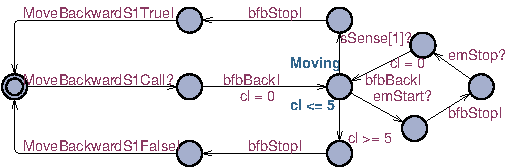
\includegraphics{MoveBackwardS1}
    \end{center}
    \caption{UPPAAL-automaat voor MoveBackwardS1. MoveBackwardS2, MoveForwardS1 en MoveForwardS2 zijn vrijwel identiek.}
    \label{fig:UPPAAL_MoveBackwardS}
    \end{figure}

    Figuur \ref{fig:UPPAAL_MoveBackwardS} is de automaat van
    MoveBackwardS1, de andere automaten lijken hier sterk op, behalve
    de richting waarin ze de band laten draaien en welke sensor ze
    controleren.

    Deze subroutine geeft de tweede lopende band opdracht in een
    bepaalde richting te gaan bewegen en komt dan in de Moving
    toestand. Vervolgens zijn er twee mogelijke uitkomsten:

    \begin{itemize}
        \item Als de lichtsensor iets waarneemt, wordt de band
        gestopt en een MoveBackwardS1True signaal aan het
        hoofdprogramma gegeven, dat aangeeft dat er inderdaad iets
        voor de sensor ligt.
        \item Als de lichtsensor na een bepaalde tijd nog niets
        gezien heeft, wordt de band gestopt en een
        MoveBackwardS1False signaal gegeven aan het hoofdprogramma
        om aan te geven dat er een time-out opgetreden is zonder dat
        de lichtsensor iets gedetecteerd heeft.
    \end{itemize}

    Een laaste mogelijkheid is nog dat er op de noodknop wordt
    gedrukt terwijl het programma in de Moving toestand is. In dit
    geval zal de band stoppen en als er weer op de noodknop wordt
    gedrukt begint de band opnieuw te lopen met de time-out weer
    teruggezet naar zijn begintoestand. In het assemblyprogramma zal
    deze time-out gewoon zijn waarde behouden.

    \subsection{Een wafer van de eerste lopende band pakken:
    LoadWafer}

    \begin{figure}
    \begin{center}
    
\includegraphics{LoadWafer}
    \end{center}
    \caption{UPPAAL-automaat voor LoadWafer.}
    \label{fig:UPPAAL_LoadWafer}
    \end{figure}

    Deze subroutine start beide lopende banden en komt dan in de
    Moving toestand. er zijn weer twee mogelijkheden om de moving
    toestand te verlaten:

    \begin{itemize}
        \item Als lichtsensor 1 iets waarneemt, ligt er blijkbaar
        een wafer klaar op band twee. Dan worden beide banden
        gestopt en krijgt het hoofdprogramma een LoadWaferTrue
        signaal om aan te geven dat er succesvol een wafer geladen
        is.
        \item Als er 10 seconden voorbij zijn en lichtsensor 1 heeft
        nog steeds niets waargenomen, lagen er blijkbaar geen wafers
        klaar op de eerste loopband. In dat geval worden beide
        loopbanden stilgezet en krijgt het hoofdprogramma een
        LoadWaferFalse signaal, om aan te geven dat er niet
        succesvol een wafer van de eerste band is gehaald.
    \end{itemize}

    Als er op de noodknop wordt gedrukt terwijl het programma in de
    Moving toestand is worden beide loopbanden gestopt. Als de
    noodknop dan weer wordt ingedrukt beginnen beide loopbanden weer
    en wordt begint de time-out weer in zijn begintoestand.\\

    Het is mogelijk dat er al een tweede wafer op de tweede lopende
    ban ligt voordat de lichtsensor de eerste detecteert. Volgens de
    opdrachtbeschrijving zouden de wafers echter met voldoende
    tussenruimte op de eerste band liggen op het moment dat er op de
    startknop wordt gedrukt en in dat geval levert dit geen
    problemen op.

    \section{Bediening deuren}

    Voor de bediening van de deuren zijn er vier subroutines, die
    verdeeld kunnen worden in twee groepen:

    \begin{itemize}
        \item Deuren openen
        \item Deuren sluiten
    \end{itemize}

    \subsection{Deuren openen: OpenDoor1, OpenDoor2}

    \begin{figure}
    \begin{center}
    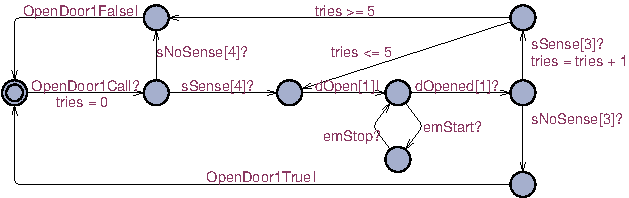
\includegraphics{OpenDoor1}
    \end{center}
    \caption{UPPAAL-automaat voor OpenDoor1. OpenDoor2 is vrijwel identiek.}
    \label{fig:UPPAAL_OpenDoor}
    \end{figure}

    In figuur \ref{fig:UPPAAL_OpenDoor} is de automaat van OpenDoor1
    afgebeeld, die van OpenDoor2 is hetzelfde, behalve dat die met andere
    sensoren en met de andere deur communiceert.\\

    Als deze routine wordt aangeroepen wordt eerst d.m.v. de
    druksensor bij deur 2 gekeken of deze deur wel echt dicht is.

    Als de deur open blijkt te zijn krijgt het hoofdprogramma een
    OpenDoor1False signaal, als de deur wel dicht is geeft deze
    routine opdracht om deur 1 te openen. Daarna controleert de
    subroutine of de deur ook echt opengegaan is d.m.v. de
    druksensor bij deur 1.

    Als de deur inderdaad open is krijgt het hoofdprogramma een
    OpenDoor1True signaal om aan te geven dat de deur succesvol
    opengemaakt is.

    Als de deur niet succesvol opengegaan is zal dit opnieuw
    geprobeerd worden, als de deur na vijf pogingen nog steeds niet
    open is krijgt het hoofdprogramma een OpenDoor1False signaal om
    aan te geven dat het openen van de deur mislukt is.


    \subsection{Deuren sluiten: CloseDoor1, CloseDoor2}

    \begin{figure}
    \begin{center}
    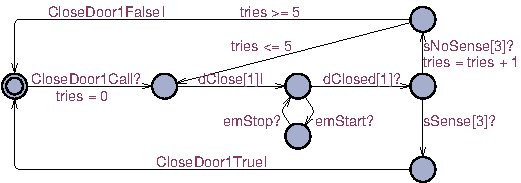
\includegraphics{CloseDoor1}
    \end{center}
    \caption{UPPAAL-automaat voor CloseDoor1. CloseDoor2 is vrijwel identiek.}
    \label{fig:UPPAAL_CloseDoor}
    \end{figure}

    Figuur \ref{fig:UPPAAL_CloseDoor} is de automaat van CloseDoor1, die van
    CloseDoor2 is identiek, behalve dat die met de andere deur en
    een andere sensor communiceert.\\

    In feite is deze subroutine ook identiek aan de
    OpenDoor-subroutines, behalve natuurlijk dat de deur hier gesloten
    wordt in plaats van geopend. Een tweede verschil is dat hier niet
    eerst wordt gecontroleerd in welke toestand de andere deur is,
    omdat het sluiten van een deur altijd is toegestaan.

    \section{Het belichten van een wafer: Burn}

    \begin{figure}
    \begin{center}
    
\includegraphics{Burn}
    \end{center}
    \caption{UPPAAL-automaat voor Burn.}
    \label{fig:UPPAAL_Burn}
    \end{figure}

    De subroutine hierboven handelt het belichten van een wafer af. In
    normale omstandigheden doorloopt deze subroutine alleen de
    onderste lus, die simpelweg de lamp inschakelt, twee seconden
    wacht, de lamp weer uitschakelt en dan een BurnTrue signaal
    geeft aan het hoofdprogramma om aan te geven dat het belichten
    goed gegaan is.

    Als echter de noodknop wordt ingedrukt terwijl de lamp aan is
    gaat de subroutine naar de bovenste lus, die in eerste instantie
    alleen maar de lamp uitschakelt. Als de noodknop weer wordt
    ingedrukt ten teken dat het systeem weer verder mag gaan zal
    de wafer naar de afvalbak vervoerd worden en vervolgens worden
    de deuren weer in de juiste stand gezet voor het verwerken van
    een volgende wafer, dus deur 2 dicht en deur 1 open. Vervolgens
    krijgt het hoofdprogramma een signaal BurnFalse om aan te geven
    dat het belichten mislukt is en dat begonnen kan worden met de
    verwerking van een eventuele volgende wafer. Merk op dat bij de
    afhandeling van deze noodstop gebruik wordt gemaakt van een
    aantal eerder in dit document behandelde subroutines.

    Als ��n van deze deuren niet goed open of dicht gaat komt de
    subroutine in de twee toestanden uiterst links en zal het
    programma crashen.

    \section{Verloren wafers afhandelen: HandleFalloff}

    \begin{figure}
    \begin{center}
    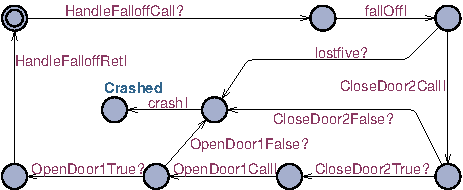
\includegraphics{HandleFalloff}
    \end{center}
    \caption{UPPAAL-automaat voor HandleFalloff.}
    \label{fig:UPPAAL_HandleFalloff}
    \end{figure}

    Als deze subroutine wordt aangeroepen wordt eerst een fallOff
    signaal gegeven aan de teller die het aantal verloren wafers
    bijhoudt. Als dan blijkt dat dit de vijfde wafer was die
    verloren ging gaat het programma naar de toestand in het midden
    en crasht het.

    Als er nog geen vijf wafers kwijtgeraakt zijn, zal deze
    subroutine zorgen dat de waferstepper klaar is om de volgende
    wafer af te handelen, dat wil zeggen: deur 2 wordt gesloten
    en deur 1 geopend. Als ��n van deze deuren niet goed open of
    dicht gaat, gaat de subroutine naar de toestanden in het midden
    en vervolgens crasht het programma.

    \section{Hulpautomaat om crashes te detecteren: ManageCrash}

    \begin{figure}
    \begin{center}
    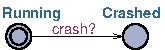
\includegraphics{ManageCrash}
    \end{center}
    \caption{UPPAAL-automaat voor ManageCrash}
    \label{fig:UPPAAL_ManageCrash}
    \end{figure}

    Zolang het programma draait zit deze automaat in de ``running''
    state. Zodra het programma ergens om een bepaalde reden crasht,
    dit kan zijn als een deur weigert te openen/sluiten of als er 5
    wafers kwijt zijn, wordt deze automaat in de ``crashed'' state
    gezet. Het nut van deze automaat is dat we gemakkelijk kunnen
    testen of het programma gecrasht is of niet, we hoeven nu
    namelijk niet alle afzonderlijke crash toestanden in de
    verschillende andere automaten te testen. 


    \chapter{Het hoofdprogramma}

    Het hoofdprogramma is gemodelleerd als een UPPAAL-template die
    de templates uit het vorige hoofdstuk aanstuurt op een zodanige
    manier dat het programma uiteindelijk doet wat het zou moeten
    doen: Het belichten van wafers en ze vervolgens in de daarvoor
    bestemde bak deponeren.\\


    \section{Het ontwerp}

    \begin{figure}
    \begin{center}
    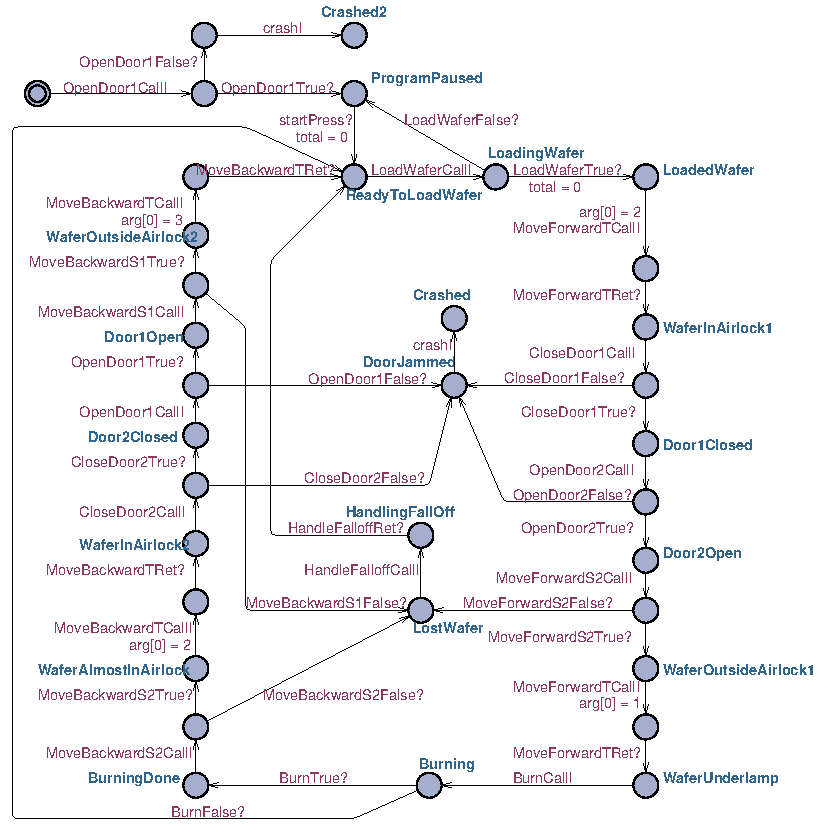
\includegraphics{Main}
    \end{center}
    \caption{UPPAAL-automaat van het hoofdprogramma.}
    \label{fig:UPPAAL_Main}
    \end{figure}

    Figuur \ref{fig:UPPAAL_Main} bevat de UPPAAL template voor het
    hoofdprogramma.

    Het eerste dat het programma doet is deur 1 openen, omdat in de
    begintoestand beide deuren gesloten zijn. Als dit mislukt crasht
    het programma onmiddellijk, anders gaat het naar de
    ProgramPaused toestand.\\

    In deze toestand wacht het programma totdat er op de startknop
    wordt gedrukt die aangeeft dat er wafers klaarliggen op de
    eerste band. Als deze knop wordt ingedrukt wordt LoadWafer
    aangeroepen. Dan wacht het programma totdat het een signaal
    terugkrijgt van deze subroutine.

    Als dit signaal LoadWaferFalse is, is er geen wafer van de eerste
    band gehaald en gaat het programma terug naar ProgramPaused,
    omdat er blijkbaar toch geen wafers klaarlagen.\\

    Als het programma een LoadWaferTrue signaal krijgt, ligt er een
    wafer klaar vlak voor de eerste deur van de luchtsluis en zal
    het programma deze wafer door de luchtsluis transporteren en
    onder de lamp leggen met behulp van de subroutines voor het
    bewegen van de lopende band en het openen en sluiten van deuren.
    Als dit alles goed gaat komt het programma in de WaferUnderLamp
    toestand.

    In dit traject kunnen echter enkele dingen misgaan. Er kan
    namelijk een deur weigeren open of dicht te gaan. In dat geval
    gaat het programma naar de DoorJammed toestand en vervolgens
    zal het crashen en in de Crashed toestand terechtkomen.

    Iets anders dat fout kan gaan is dat de wafer de tweede
    lichtsensor niet bereikt op het moment dat dat wel zou moeten.
    In dat geval wordt geconcludeerd dat de wafer verloren is gegaan
    en gaat het programma naar de LostWafer toestand. Daarna zal
    HandleFalloff aangeroepen worden. Als deze routine returnt is
    het systeem klaar om de volgende wafer te verwerken en gaat het
    programma naar ReadyToLoadWafer.\\

    Als alles echter goed gaat, ligt de wafer op dit moment onder de
    lamp en wordt er een aanroep gedaan naar Burn. Dit zorgt er in
    principe voor dat de wafer belicht wordt en dat het
    hoofdprogramma een BurnTrue signaal krijgt.

    Als er echter tijdens het belichten een noodstop plaatsvindt
    krijgt het hoofdprogramma een BurnFalse signaal. In dit geval is
    het systeem klaar voor het verwerken van de volgende wafer en
    gaat het programma dus terug naar ReadyToLoadWafer.\\

    Als alles goed gaat tijdens het belichten komt het programma in
    de toestand BurningDone. Vervolgens wordt de wafer door de
    luchtsluis naar de opvangbak getransporteerd. Dit proces en de
    zaken die hierbij mis kunnen gaan zijn vergelijkbaar met het
    naar binnen brengen van de wafer en zal hier ook niet verder
    toegelicht worden.\\

    Als de wafer in de bak ligt komt het systeem in toestand
    ReadyToLoadWafer en zal proberen de volgende wafer van de eerste
    band te halen. Als dit lukt begint het hele verhaal weer
    opnieuw, anders zijn blijkbaar alle wafers verwerkt en dan gaat
    het programma naar de ProgramPaused toestand, waar het wacht tot
    er op de startknop wordt gedrukt om aan te geven dat er weer
    wafers klaarliggen.


\end{document}


\chapter{Systeemanalyse}


    \section{Inleiding van de systeemanalyse}
        Bij de systeem analyse controleren we of ons UPPAAL-model correct is. Om dit te controleren moeten
        we eerst defini\"eren wat we verstaan onder ,,correct''. Wij zullen dit defini\"eren met
        behulp van eigenschappen waaraan ons systeem dient te voldoen; wanneer dit het geval is, achten
        wij het systeem correct. Deze eigenschappen zullen we toelichten, vertalen naar UPPAAL-queries, en
        testen volgens het verificatiesysteem van UPPAAL zelf. De resultaten zullen we ook evalueren in dit
        document.


    \section{Belangrijke eigenschappen functionaliteit}
        Hieronder is beschreven aan welke eigenschappen ons systeem moet voldoen. Het vierde item kan echter niet
        gegarandeerd worden bij indrukken van de noodknop; met deze uitzondering zal bij de simulatie en verificatie
        rekening worden gehouden.
        \begin{enumerate}
            \item Er zijn nooit twee deuren tegelijk open.
            \item De lamp is alleen aan bij belichten van een wafer.
            \item Vlak voordat een wafer aan ,,zijn cyclus'' begint is deur \'{e}\'{e}n open en deur twee dicht.
            \item Voor alle paden geldt dat een wafer binnen twintig seconden in een bak ligt of verloren is gegaan, mits er niet
                  op de noodknop wordt gedrukt.
            \item Het systeem crasht alleen wanneer het moet crashen.
        \end{enumerate}

    \section{Methodiek simuleren en verifi\"eren eigenschappen}
        Voor het simuleren van het systeem gebruiken wij de Simulator welke in UPPAAL beschikbaar is. Deze
        laten we random acties simuleren op de hoogste snelheid voor een duur van maximaal vijf minuten. Dit
        proces herhalen we enkele malen om er zeker van te zijn dat ons systeem inderdaad geen deadlocks bevat.\\
        \\
        Bij het verifi\"eren maken wij gebruik van z.g.n. queries, welke uitdrukken wat precies wij willen
        verifi\"eren. De nummering is gelijk aan die van de vorige lijst:
        \begin{enumerate}
            \item A[] (door1.Closed or door1.PseudoClosing or door2.Closed or door2.PseudoClosing)\\
                \emph{    Er moet altijd gelden dat er minstens \'{e}\'{e}n deur gesloten is. De toestandsnaam PseudoClosing
                            zou kunnen impliceren dat de deur aan het sluiten is; dit is echter een tussentoestand
                            in UPPAAL en in feite is de deur dan al gesloten.}
            \item A[] (lamp.On) imply (main.Burning)\\
                \emph{    Als de UV-lamp aanstaat, moet gelden dat er een wafer wordt gebrand.}
            \item A[] main.ReadyToLoadWafer imply (door1.Open and door2.Closed)\\
                \emph{    Voordat er een wafer wordt geladen, staat deur \'{e}\'{e}n open en is deur twee gesloten. ``main'' is de naam
                van het hoofdprogramma.}
            \item A[] main.ReadyToLoadWafer imply (main.total $<$= 15)\\
                \emph{    Voordat er een nieuwe wafer wordt geladen en dus de vorige reeds klaar is, moet
                            gelden dat het aantal verstreken seconden niet hoger is dan 15 sinds laden van
                            die wafer.}
            \item A[] managecrash.Crashed or not deadlock\\
                \emph{    Het systeem is ofwel in een crash-toestand, of draait zoals normaal.}
        \end{enumerate}

    \section{Simulatie- en verificatieresultaten}
        Volgens de eerste beschreven methode hebben wij het systeem gesimuleerd. Formeel zijn de resultaten hieronder
        beschreven. Informeel komt het erop neer dat al onze simulaties goed zijn verlopen en we dus ons systeem als
        correct mogen beschouwen. Helaas komt het regelmatig voor (dankzij UPPAAL's testsysteem) dat de deuren vast-
        lopen en komt daardoor in een crash-toestand. Dit is echter de bedoeling wanneer een deur vastloopt, dus is
        een resultaat van deze aard een gewenst resultaat.\\
        \\
        \begin{tabular}{ c | l | c }
            Duur & Opmerkingen & Resultaat\\
            \hline
            9s & deur weigert -$>$ crash & succesvol\\
            2s & deur weigert -$>$ crash & succesvol\\
            1s & deur weigert -$>$ crash & succesvol\\
            5s & deur weigert -$>$ crash & succesvol\\
            4s & deur weigert -$>$ crash & succesvol\\
        \end{tabular}\\\\
        \\
        Volgens de tweede beschreven methode hebben wij het systeem geverifi\"eerd. Bij al onze opgegeven queries
        gaf het systeem het resultaat ,,Property is satisfied'', wat dus inhoudt dat in alle gevallen het systeem
        voldoet aan de opgegeven eigenschappen.\\

    \section{Conclusie van de systeemanalyse}
        We kunnen dus concluderen dat ons systeem voldoet aan de gestelde eisen en eigenschappen.


\chapter{Testresultaten}
\section{Testresultaten en problemen}
Wij hebben ons systeem natuurlijk ook getest. Hier volgen enkele tests die wij uitgevoerd hebben, samen met de resultaten hiervan. Daarnaast hebben we hier ook een paar problemen aangestipt die we onderweg tegenkwamen.

\subsection{Problemen en mislukte tests}
We beginnen met de problemen die we zijn tegengekomen en hoe we deze overwonnen hebben.

\begin{itemize}
    \item Lampjes: Hier hebben we toch wel wat problemen mee gehad, voooral omdat de lampjes eigenlijk op 12 volt werken. De enige aansluitingen die we hadden op de processor waren +5V, +16V en ground. 16 volt bleek te veel, de lampjes werden erg warm, wat de behuizing niet ten goede kwam. Een combinatie van 5 en 16 volt (resulterend in 11 volt) leek een goede keus, maar de processor vertoonde op slag kuren. Na wat meetwerk kwamen we erachter dat de 5 volt van de processor op deze manier omhooggetrokken werd tot 7 volt - dit kon nooit goed zijn. Hierna hebben we er voor gekozen om de lampjes toch maar op 5 volt aan te sluiten.
    \item Sensoren (1): De sensoren hebben ons vrij veel problemen opgeleverd. Het eerste probleem was dat de sensoren aangesloten waren op een input-poort en de +5 volt. Aangezien de processor pull-up weerstanden heeft, kon het verschil tussen wel of geen actie niet waargenomen worden. Dit was gelukkig vrij makkelijk te verhelpen door de sensoren aan te sluiten op de ground in plaats van de +5 volt.
    \item Sensoren (2): Omdat de lampjes niet op volle kracht werkten, konden we het verschil in lichtsterkte niet direct meten. In het begin hadden we het idee om een comparator tussen de sensoren en de processor te zetten, zo hoeven we niet in software de sensoren te ijken. We hadden in het begin de lampjes op 16 volt aangesloten, waarbij de comparator niet meer nodig was. Uiteindelijk hadden we de lampjes op 5 volt aangesloten en zijn weh dus toch maar comparators gaan halen, samen met een potmeter om de spanning in te stellen.
    \item Sensoren (3): Zelfs met comparator waren de sensorwaarden niet uitleesbaar, deze keer omdat de spanning over de sensor gelijk bleef, alleen de weerstand veranderde. We hadden dus nog twee weerstandjes nodig die de verhouding van de spanning zou veranderen. Na deze weerstandjes toegevoegd te hebben konden we eindelijk de sensoren uitlezen.
    \item Noodknop: De subroutine die de noodknop in de gaten hield gaf problemen: zodra dit bestand opgenomen werd in het hoofdprogramma en er op de noodknop gedrukt werd, reageerde TScope niet meer. Na de code goed nagekeken te hebben bleek dat de afhandeling van de interrupt niet correct was. 
    \item Compressormotor: De motor van onze compressor is aangesloten op 16 volt. Dit zorgt natuurlijk voor de nodige luchtdruk, maar het heeft ook een nadeel: de motor en de aandrijfassen trillen aanzienlijk. Hierdoor bleven de wafers niet goed liggen tijdens het branden en verdwenen zij weer in de luchtsluis. Dit probleem was na enig nadenken verholpen door een verstevigende balk tegen het motorblok aan te brengen. De trilligen zwakten af en er kon normaal gewerkt worden.
\end{itemize}

\subsection{Geslaagde onderdelen}
Hier volgen de onderdelen die functioneerden zoals we gehoopt hadden, zonder al te veel aanpassingen.

\begin{itemize}
    \item Motoren: De motoren van de lopende banden waren vrij makkelijk in te stellen. We hadden verwacht dat we Pulse Width Management moesten gebruiken om de juiste snelheid van de banden te bepalen en na een korte test op volle kracht bleek dit ook waar te zijn. Na een kleine verandering in de code liepen de banden perfect.
    \item Deuren: Naast een paar luchtslangen die zo nu en dan losschoten deden de deuren het goed. De kleppen reageerden netjes op het programma en de druksensoren gaven (na de aanpassingen zoals hierboven beschreven) de goede waardes terug.
    \item Verloren Wafers: Ook deze tests verliepen goed. Zodra een wafer als verloren is gemarkeerd springt een extra LED op het processorbordje aan. Als de vijfde wafer verloren is gegaan crasht het programma.
    \item Daarnaast waren grote onderdelen van de programmatekst vrijwel meteen goed geschreven. Het UPPAAL-ontwerp heeft hier natuurlijk ook ontzettend aan bijgedragen, maar toch liep alles veel soepeler dan we verwacht hadden.
\end{itemize}

\chapter{Procesdocument}
\section{Tijdverdeling}
Iedereen heeft een logboek bijgehouden op een online systeem
tue.coenvdwel.com/lbs. Deze logboeken zijn in de bijlage te vinden.

\subsection{Vergadering} De vergadering werd elke
donderdagmiddag gehouden en duurde ongeveer een half uur.

\section{Taakverdeling}
\subsection{Voorzitter, Notulist}
Wie er voorzitter en notulist waren tijdens de vergadering
veranderde per week. Iedereen is minstens \'{e}\'{e}n keer
voorzitter en \'{e}\'{e}n keer notulist geweest.

\begin{tabular}{|c | c | c | c|}
      \hline
      id-nummer & naam & voorzitter & notulist\\
      \hline
      0618959 & Etienne van Delden & week 13 & week 14 en 21\\
      0611093 & Gijs Direks & week 14 en 21 & week 15 en 20\\
      0588898 & Sanne Ernst & week 15 en 22 & week 16 en 23\\
      0598669 & Bas Goorden & week 16 en 23 & week 17 en 22\\
      0607426 & Stef Sijben & week 17 & week 18\\
      0608467 & Coen van der Wel & week 18 en 20 & week 14\\
      \hline
\end{tabular}

\subsection{Werkplan}
\subsubsection{Mechanisch }
  \begin{itemize}
    \item Ontwerp (Gijs)
    \begin{itemize}
        \item Schets
        \item Specificatie technische details
    \end{itemize}
    \item Bouwen ontwerp (Sanne)
  \end{itemize}

\subsubsection{Software}
  \begin{itemize}
    \item Schrijven basis (Stef)
    \begin{itemize}
        \item I/O subroutines
        \item Interrupt handlers
    \end{itemize}
    \item Aansturen mechanisch ontwerp (Coen)
    \begin{itemize}
        \item Index-based
    \end{itemize}
  \end{itemize}

\subsubsection{Misc.}
  \begin{itemize}
    \item Documentatie (hele groep)
    \item Demonstratie met uitleg (Etienne)
    \item Handleiding (Bas)
    \item Verslag (Bas)
  \end{itemize}

\subsubsection{Deadlines}

    \begin{tabular}{l | c | c | c | c }
      Onderdeel & Verantwoordelijke & Start datum & Interne deadline & Externe deadline\\
      \hline
      Ontwerp en operationele specificatie & Gijs/Etienne & 26-03 & 18-04 & 23-04  \\
      ~~~ UPPAAL & Gijs & 26-03 & 16-04*&23-04\\
      ~~~ Tekeningen (foto's) & Etienne & 26-03 & 18-04 &23-04\\
      Specificatie elektrische interface & Gijs/Sanne & 26-03 & 23-04* & 23-04 \\
      ~~~ Bedradingsschema & Gijs & 26-03 & 16-04* & 23-04\\
      ~~~ Model (hardware) & Sanne & 26-03 & 23-04\\
      Programma ontwerp (UPPAAL) & Stef & 16-04 & 23-04* & 01-05\\
      Systeem analyse (UPPAAL) & Coen & 23-04 & 27-04 & \\
      Implementatie & Stef/Coen & 23-04 & 21-05* & 29-05 \\
      ~~~ Assembler code&Stef&23-04 & 21-05* & 29-05\\
      ~~~ Aansturen mechanisch ontwerp &Coen&23-04 & 21-05* & 29-05\\
      Verslag en documentatie & Bas & 26-03 & 04-05* & 11-06\\
      Demonstratie met uitleg & Etienne & 30-05 & n.v.t. & 14-06\\

    \end{tabular} \\ \\
*voor 12.00 uur inleveren

\section{Evaluatie}
\subsection{Persoonlijke evaluatie van Etienne van Delden}

    Dit was voor mij de derde ogo, met als grootste verschil dat we twee
    dubbele P-ers en twee minoren in het groepje hadden. Dit maal kwamen
    onze roosters dus niet overeen. Hierdoor moesten we af en toe door werken met minder mensen als normaal.
    Ook verschilde de ervaringen met (OGO) groepsprojecten, waardoor
    we in het begin een moeilijke start hadden. Sommige dingen die voor Coen en mij logisch waren,
    zoals verslagen op studyweb zetten, waren voor de anderen nog niet logisch.
    Gelukkig was alles goed gekomen, toen we duidelijker afspraken maakten, alles goed gingen
    doorspreken en ikzelf aangesteld werd als quality-manager. \\

    Ik heb mij vooral bezig gehouden met het hardware-model. Ik heb
    meegeholpen aan de bouw ervan en ik heb de scart-interface
    grotendeels aangesloten. Het aansluiten van de scart-interface om het
    processorbord en het model makkelijk aan te sluiten was mijn idee. Hoewel het
    zeker voordelen heeft, hebben we hierdoor wel veel tijd
    verloren. Het aansluiten van alle 24 kabels duurde langer als verwacht \'e er waren een aantal fouten gemaakt,
     Gelukkig is alles nog gelukt met de scart aansluiting. \\

    Ook was ik verantwoordelijk voor de presentatie. Hoewel ik op
     moment van schrijven nog niets kan zeggen over de presentatie
      op de laatste ogo dag, samen met de
    demonstratie, had ik de eindpresentatie wel al gebruikt bij de
    presentatie training. Coen van der Wel en ikzelf hebben daar de
    eindpresentatie gegeven, waarbij die als erg goed werd
    beoordeeld.`\\

    Hoewel ik vrij weinig code heb geschreven, heb ik wel veel
    geleerd over de problemen die onstaan bij het maken van een
    embedded systeem. Voor het eerst hebben we eerst een model in
    UPPAAL gemaakt, van zowel het hardware als het software model,
    en pas daarna gewerkt aan de software zelf. We hebben daarbij
    ondervonden dat dit enorm helpt, omdat je dan een richtlijn hebt
    voor hoe je code moet worden. \\

    Qua verantwoordelijkheid wou ik me meer op de achtergrond houden,
    uit vorige ogo's heb ik gemerkt dat ik soms me teveel
    met anderen bemoei. Dit was toch niet helemaal gelukt. Door de
    moeilijke start werd ik uiteindelijk aangesteld als
    quality-manager, waarbij ik de verantwoordelijkheid draag voor
    de ingeleverde documenten. Mijn taak resulteerde uiteindelijk
    tot externe agenda voor de anderen. Ik hoefde zelf niet
    opdrachten te geven, maar mij werd gevraagd wat er moest
    gebeuren. Dit maakte het voor mij prettiger, omdat ik niet opdrachten hoef uit te geven
    , maar ook voor de anderen die een vraagbaak haddden en iemand die wist wat er allemaal moest gebeuren. \\

\subsection{Persoonlijke evaluatie van Gijs Direks}

Dit was mijn eerste OGO, mijns inziens ook een zeer geslaagde.
Na een paar opstartproblemen, vooral te wijten aan het feit dat
maar twee personen al eerder OGO gehad hebben, liep alles lekker
 door. We hebben met zes man hard en goed gewerkt aan dit project.\\
\\
Ik heb ook veel geleerd van deze OGO. Naast het omgaan met andere
mensen was er natuurlijk ook het technische aspect. Fischertechnik
is natuurlijk geen ontzettend hoogstaand materiaal en brengt menige
beperking met zich mee, maar dit levert ook uitdagingen die
overwonnen moeten worden. Enkele van deze problemen vergden 'nieuwe'
oplossingen, die een andere kijk met zich meebrachten.\\
\\
Ook de practicumprocessor heeft enkele kopzorgen gebaard: bij het
ontwerp van de elektrische interface had ik er bijvoorbeeld geen
rekening mee gehouden dat er pull-up weerstanden aan de poorten
zitten - dit had als effect dat ik de noodknop en de sensoren op een
ingangspoort en +5V aangesloten had. De processor las dan ook geen
bruikbare waarden uit.
Na een opmerking van Stef en wat solderen was dit toch weer snel verholpen.\\
\\
Al met al vond ik dit een zeer geslaagde OGO, het was een interessant probleem en ik heb met leuke mensen samengewerkt.

\subsection{Persoonlijke evaluatie van Sanne Ernst}

Bij wiskunde heb ik modelleervakken gevolgd, daarentegen was OGO
voor mij nieuw. In plaats van werken in groepjes van twee moesten we
nu met zes man werken. Dit maakt het werken in een groep een stuk
gezelliger en je bent ook niet gebonden aan \'e\'en partner.
Dit was voor mij een nieuwe en ook prettige ervaring. \\

Wat voor mij totaal nieuw was, waren de wekelijkse vergaderingen.
Hierbij heb ik het belang van vergaderen geleerd, namelijk het
periodieke spreken van de opdrachtgever. Echter vond ik de
vergaderingen te formeel en over het algemeen te lang duren.\\

Voor OGO 1.3 had ik nog niet zoveel ervaring met het ontwerpen en
maken van programmatuur. Ik had wel al ervaring met het programmeren
van java-applicaties bij modelleren. Nu ben ik voor het eerst
begonnen met het maken van een model alvorens de applicatie zelf te
maken. Dit werkte zeer prettig, omdat ik nu een richtlijn had voor
het schrijven van code. Ook heb ik meer ervaring opgedaan met het
schrijven van assembler code.\\

Verder heb ik meegeholpen met het bouwen van het hardware-model. Dit
vond ik heel erg leuk om te doen, omdat dit een heel gepuzzel was.
De vorm van de stukjes maakt het soms lastig om te bepalen wat het
doel ervan is. Het werken met Fischertechnik deed mij denken aan
het spelen met Lego. Wat ik onder andere ontworpen heb zijn de lopende banden.\\

Hoewel we een moeilijke start hadden, werd het uiteindelijk een heel
geslaagde OGO.

\subsection{Persoonlijke evaluatie van Bas Goorden}

Dit was ook voor mij de eerste OGO. De major die ik volg is
Technische Wiskunde en dit was \'{e}\'{e}n van de vakken die ik in
mijn minor gekozen heb. \\

Bij wiskunde hebben we intussen toch al een behoorlijk aantal
Modelleren-projecten gedaan. Hierdoor was ik bang dat ik aan dit
vak, op het gebied van samenwerken, weinig zou hebben. Het feit dat
de groepen bij dit vak uit zes in plaats van uit twee personen
bestaan had echter zijn gevolgen. Bij Modelleren weet je namelijk
altijd precies wat er gebeurt en als je zelf niks doet gebeurt er
ook niks. Het was daarom zaak om in de gaten te houden waar de rest
van de groep mee bezig was en om daar vragen over te stellen als zij
iets gedaan hadden wat ik nodig had. Daarnaast ben je, als je deel
uitmaakt van een groep van twee personen, zelf betrokken bij en
verantwoordelijk voor alle belangrijke beslissingen. Bij OGO was dit
niet zo, onze groep bestond namelijk voornamelijk uit mensen die
geen enkel probleem hebben met het nemen van belangrijke
beslissingen. Hier heb ik mij aan aangepast, door mezelf niet bij
alle belangrijke beslissingen te betrekken. Dit viel mij minder
zwaar dan ik verwacht had. Ik heb bij dit OGO-project dus eens een
andere manier van samenwerken meegemaakt en dat heeft zeker een
bijdrage geleverd aan mijn vaardigheden op dat gebied.\\

Wat natuurlijk ook belangrijk is, is dat ik veel geleerd heb wat de
informatica zelf betreft. Ik heb mij eigenlijk een beetje met alle
belangrijke onderdelen van dit project beziggehouden. Eerst met het
bouwen van het hardware-model, vervolgens met het maken van een
programmaontwerp in UPPAAL, daarna met het schrijven van een aantal
subroutines en tot slot met het verslag. Vooral van het maken van
het programmaontwerp en van het schrijven van code heb ik veel
geleerd. Met de presentatie heb ik mij helemaal niet beziggehouden,
maar bij Modelleren heb ik al een behoorlijk aantal presentaties
gehouden, dus ik denk niet dat dat erg is.\\

Al met al heb ik er dus veel van geleerd. Het is niet meer dan de
kers op de taart, maar toch het vermelden waard, dat ik het
onderwerp van het project interessant vond en dat de samenwerking
binnen de groep goed was. Al met al was dit dus een geslaagde OGO.\\

\subsection{Persoonlijke evaluatie van Stef Sijben}

Deze OGO begon enigszins moeizaam, waarschijnlijk mede doordat in
onze groep slechts twee personen waren die al eerder een OGO hadden
gedaan. Na een aantal weken ging het echter beter en vanaf dat
moment zijn er weinig grote problemen meer geweest. De samenwerking
met de rest van de groep is in het algemeen goed verlopen.\\

Het gebruik van Fischertechniek bracht de nodige beperkingen met
zich mee, maar het was een leuke uitdaging om hier omheen te werken,
mede omdat we graag wilden proberen de hele waferstepper op \'e\'en
bordje te bouwen.

Daarnaast hebben we geleerd dat het bij een eventueel volgend
project handig is om de elektrische aansluitingen wat beter te
organiseren. Nu waren er namelijk nogal wat draden fout aan elkaar
gesoldeerd, waardoor het model niet goed werkte.\\

Ondanks dat ik al de nodige ervaring had met embedded systemen, heb
ik op dit gebied toch ook nog de nodige dingen geleerd omdat deze
processor op sommige gebieden nogal verschillend is van de
processoren waar ik tot nu toe mee gewerkt heb.\\

Omdat ik intensief gewerkt heb aan het ontwerp van de
UPPAAL-modellen heb ik ook op het gebied van specificeren veel
nieuwe dingen geleerd, ik was hiermee namelijk nog niet eerder in
aanraking gekomen.\\

Met de presentatie heb ik me niet beziggehouden, maar ik heb wel al
een presentatie gedaan voor modelleren, dat ik in blok D gevolgd heb
in het kader van de dubbele propedeuse die ik doe. Ik denk dan ook
dat dat niet echt een probleem zal zijn.\\

Wel heb ik het nodige geleerd van verslaglegging, ik heb namelijk
het verslag van het programmaontwerp grotendeels geschreven. De
verslaglegging daarvan is toch wel anders dan andere verslagen die
ik tot nu toe geschreven heb.\\

Deze OGO is in mijn ogen dus goed verlopen en ik heb er veel van
geleerd.//

\subsection{Persoonlijke evaluatie van Coen van der Wel}

    Persoonlijk vond ik dit een geslaagde OGO. Vanwege een kleine
    miscommunicatie in het begin was er even een probleem met het
    samenstellen van de groepen, maar uiteindelijk werd de groep
    samengesteld uit 3 van mijn vrienden en 2 minor-studenten, waarmee
    ik inmiddels ook goed overweg kan. Ik denk dat dat zeker heeft
    bijgedragen aan het resultaat, want een goede relatie met collega's
    is ook echt belangrijk.\\
    \\
    Verder heb ik veel geleerd over pneumatiek en electrische
    interfaces, ik heb zeker mijn deel bijgedragen aan het uitwerken van
    deze twee dingen. Ook heb ik mijn LEGO \texttrademark \ ervaring uit kunnen
    breiden door het bouwen van het model met Fischertechnik \texttrademark \. De
    beperktheden van deze techniek leidden tot een meer gecompliceerd
    model, maar die uitdaging is juist leuk. Het programmeren van het
    model en het kennismaken met een embedded systeem is uiteraard ook
    een belangrijk aspect geweest en heb ik met veel plezier gedaan.\\
    \\
    De presentatie heeft Etienne grotendeels verzorgd, maar hierbij heb
    ik toch zeker geen onbelangrijke rol gespeeld. De
    presentatietraining was voor mij niet echt nuttig, ik heb er namelijk
    niet erg veel van geleerd. Het rapporteren en verslagleggen van
    (tussen)resultaten was zoals bij de vorige OGO's een beetje een blok
    aan het been, maar gaat naar mijn mening wel steeds beter. Ik ontken
    dan ook niet dat deze verslagen nuttig zijn, maar het spelen met het
    model is natuurlijk veel leuker ;-)\\
    \\
    Qua verantwoordelijkheden heb ik mezelf een beetje teruggetrokken. Bij
    vorige OGO's is mijn ervaring dat ik me met alles bemoei en dat uiteindelijk
    alles op mij neerkomt; bij deze OGO heb ik me meer afzijdig gehouden, met de
    keerzijde dat ik me niet erg nuttig heb gevoeld. Er moet vast een tussenweg
    zijn... dat als verbeterpunt voor mezelf voor een volgende OGO.\\
    \\
    Maar al met al vind ik het een geslaagde OGO!



\chapter{Conclusie}
\section{Conclusie}

Na drie maanden hard werken en een moeilijke start, is onze Prime Waferstepper af. We hebben allemaal hard samengewerkt om een goed werkend en compact model van een waferstepper te maken dat, naar onze mening, voldoet aan de gegeven eisen.\\

Het gebruik van de SVN server heeft onze samenwerking goed bevorderd, iedereen had de nieuwste versie van een verslag of code. Niet iedereen had hier ervaring mee, maar al heel snel werd dit systeem goed gebruikt en geprezen. \\

Om de software op de processor te zetten moesten wij gebruik maken van tScope. Dit programma is naar onze mening zeer onstabiel, op het moment dat het crashed moet je je computer opnieuw opstarten. Ook het feit dat het crasht na interrupt handling, dat bij de noodknop essentieel is, heeft voor veel frustratie gezorgd. \\

Ondanks alle tegenslagen, hebben we allemaal veel geleerd over het maken van een embedded system. Ook hebben wij kennisgemaakt met UPPAAL en hebben wij allen het nut van het maken en controleren van een model voorgaande aan het programmeren zelf ondervonden. Dit brengt structuur in de manier van werken.\\




\newpage
\appendix

\chapter{Assembler code}
\section{main}


\begin{verbatim}
TITLE 'Main Program' SBTTL 'OGO1.3 group 7, 2006-2007' ; ; This is
the main module of the waferstepper controller. It implements the
following subroutines: ; Crash: A 'subroutine' that will loop to
itself forever. ; Labels used are (mostly) equivalent to those in
the UPPAAL model. Bootup:
        ORG     00h
        AJMP    main                    ;Skip reserved memory


        ;   skip first bytes + includes
        INCL 'int_vect.asm'

        ORG 0080h
        INCL 'mem_subs.asm'
        INCL 'wt_subs.asm'
        INCL 'iol_subs.asm'
        INCL 'ioh_subs.asm'
        INCL 'emergenc.asm'
        INCL 'init.asm'

main:   ;Start of program
        MOV     SP, #8
        ACALL   init                    ;Initialise all components to their desired states.

ProgramPaused:
        MOV     DPTR, #0FF00h           ;The adress of the dip-switches, of which switch 0 is the 'ready button'
        MOVX     A, @DPTR
        JNB     Acc.0, ProgramPaused

        ;Ready  button has beed enabled.

ReadyToLoadWafer:
        ACALL   LoadWafer               ;Loads a wafer. C = 1: succes, C = 0: Failure
        JNC     ProgramPaused

        ;We want to move the wafer forward for 1 second
        MOV     A, #20d
;TODO: check the timing of this!
        ACALL   MoveForwardT

        ACALL   CloseDoor1
        JNC     DoorJammed              ;Check whether the door actually closed

        ACALL   OpenDoor2
        JNC     DoorJammed              ;Check whether the door actually opened

        ACALL   MoveForwardS2           ;Moves the wafer to the sensor
        JNC     WaferLost               ;Check whether wafer has arrived

        MOV     A, #10d
;TODO: check the timing of this!
        ACALL   MoveForwardT            ;move wafer under UV lamp
        ACALL   Burn                    ;burn the wafer
        JNC     ReadyToLoadWafer

        ACALL   MoveBackwardS2          ;move wafer back to sensor
        JNC     WaferLost

        MOV     A, #20d
;TODO: check the timing of this!
        ACALL   MoveBackwardT

        ACALL   CloseDoor2              ;Closes door 2
        JNC     DoorJammed              ;Check whether door has closed

        ACALL   OpenDoor1               ;Opens door 1
        JNC     DoorJammed              ;Check whether door has opened

        ACALL   MoveBackwardS1          ;Move wafer to sensor 1
        JNC     WaferLost               ;Check whether wafer has arrived

        MOV     A, #60d
;TODO: check the timing of this!
        ACALL   MoveBackwardT           ;Move burnt wafer off the belt

        AJMP    ReadyToLoadWafer

;This state is reached when a door is stuck. It moves to Crash.
DoorJammed:
        AJMP    CrashMain

CrashMain:
        AJMP    CrashMain               ;Program Crash, restart required.

WaferLost:
        ACALL   LostWafer               ;This wafer is lost, prepare for handling the next one
        AJMP    ReadyToLoadWafer        ;And then start handling the next one if possible

        END Bootup
\end{verbatim}



\chapter{Logboeken}
Op de volgende pagina's staan de logboeken van alle groepsleden (in
alfabetische volgorde).

\begin{figure}
\begin{center}
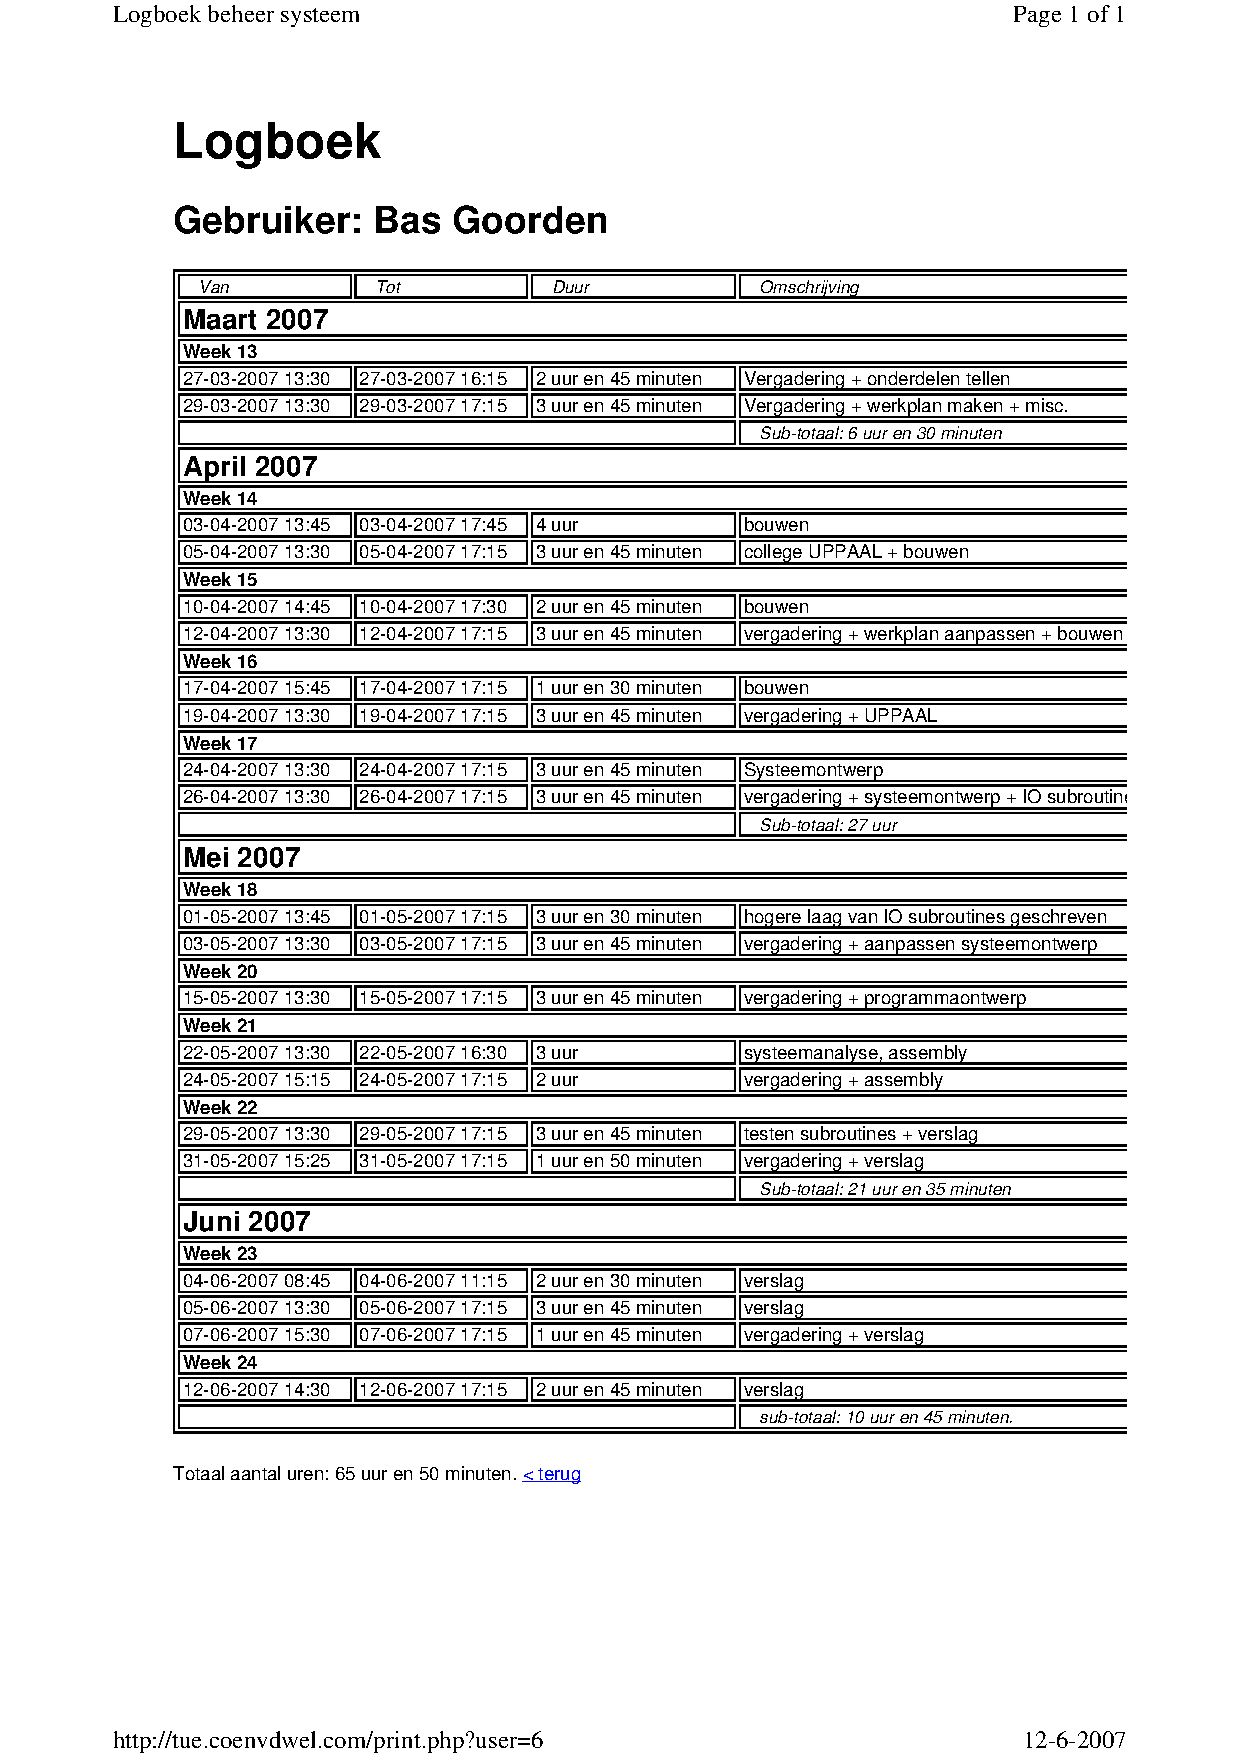
\includegraphics[width=1\linewidth]{logboekbas}
\label{bas}
\end{center}
\end{figure}

%\chapter{Begrippenlijst}
%\input{begrippenlijst}


% De bibliografie
%\input{bibliografie}



% section a (end)



\end{document}
